\documentclass[12pt,twoside]{report}
\usepackage{lmodern} % Fuente similar a Computer Modern pero mejorada
\linespread{1.1} % Aumenta un poco el interlineado

% Paquetes necesarios
\usepackage[acronym]{glossaries}  
\usepackage[utf8]{inputenc}
\usepackage[T1]{fontenc}     % Codificación de fuentes
\usepackage[spanish]{babel}
\usepackage{geometry}        % Controlar márgenes
\usepackage{titlesec}        % Personalizar títulos de capítulos y secciones
\usepackage{hyperref}        % Enlaces en el PDF
\usepackage{graphicx}        % Insertar imágenes
\usepackage{adjustbox}
\usepackage{float}
\usepackage[backend=biber, style=numeric]{biblatex}
\usepackage{csquotes}
   % Glosario
\makeglossaries
\addbibresource{bibliografia.bib}

\titlespacing*{\chapter}{0pt}{0.5cm}{0.5cm} % Ajustar espaciado en cm


% Configuración de márgenes
\geometry{
    a4paper,
    left=3cm,
    right=2.5cm,
    top=2.5cm,
    bottom=2.5cm
}

\newglossaryentry{vulnerabilidad}{
    name=vulnerabilidad,
    description={una debilidad común y recurrente que ocurre debido a errores en el
desarrollo, poco control de calidad en las etapas del SDLC o poca preocupación por cuestiones
de seguridad. Esto sumado a la práctica de compartir información y conocimiento que tiene la
comunidad de ciberseguridad, les permite a los hackers aprovecharse de estas vulnerabilidades.}
}

\newglossaryentry{patrón}{
    name=patrón,
    description={Es una solución general a un problema recurrente en un contexto determinado. En
el desarrollo de software, un patrón es una solución probada y documentada a un problema}
}

\newglossaryentry{antipatrón}{
    name=antipatrón,
    description={Es una mala práctica de software. describe una solución común a un pro-
blema frecuente, pero que genera consecuencias negativas. Deja al descubierto como algunas
prácticas comunes en el desarrollo de software parecen apropiadas pero en realidad introducen
más vulnerabilidades.}
}

\newacronym{cms}{CMS}{Content Management System}
\newacronym{cve}{CVE}{Common Vulnerabilities and Exposures}
\newacronym{cwe}{CWE}{Common Weakness Enumeration}
\newacronym{vap}{VAP}{Vulnerability Antipattern}
\newacronym{api}{API}{Application Programming Interface}
\newacronym{sdcl}{SDLC}{Software Development Life Cycle}
\newacronym{sql}{SQL}{Structured Query Language}

% Documento
\begin{document}

% portada.tex
\begin{titlepage}
\begin{center}

\begin{center}
    
\includegraphics[height=2.5cm]{Imagenes/logofcefynunc.png}
\end{center}


\vspace{2cm}

\textbf{\large UNIVERSIDAD NACIONAL DE CÓRDOBA} \\[0.3cm]
\textbf{\large FACULTAD DE CIENCIAS EXACTAS, FÍSICAS Y NATURALES} \\[3cm]

\textbf{\huge Antipatrones de Seguridad en WordPress:} \\[0.3cm]
\textbf{\huge Diseño de una API para su Detección y Mitigación} \\[0.8cm]

\textit{\large Proyecto Integrador de Grado de Ingeniería en Computación} \\[2cm]

\begin{minipage}{1\textwidth}
    \centering
    \textbf{\Large COMMISSO, Gina} 
\end{minipage}

\vspace{2cm}

Dirigido por \\
Mgter. Ing. \textbf{SOLINAS}, Miguel \\[0.5cm]

Codirigido por \\
Ing. \textbf{JORGE}, Javier \\[3cm]

\textbf{27 de junio 2025}

\end{center}
\end{titlepage}




\thispagestyle{empty}  % sin número de página

{\LARGE Agradecimientos}


\vspace{2cm}

\begin{center}
\textbf{Resumen}
\end{center}

\vspace{2em}
Las vulnerabilidades definen la superficie de ataque de un sistema digital. Incluso en su configuración mínima, una aplicación expuesta a redes públicas o privadas incluye múltiples capas como firmware, sistema operativo, frameworks y aplicaciones con arquitecturas propias, todas susceptibles a vulnerabilidades conocidas y registradas en bases como \ACRshort{cve} \cite{CVE}. A pesar de contar con información pública sobre estas fallas, es común que se repitan en nuevos desarrollos.

Este trabajo parte de esa contradicción: ¿por qué las vulnerabilidades conocidas siguen ocurriendo? En contextos donde prima la entrega rápida de funcionalidad y hay poca formación en ciberseguridad, las buenas prácticas se relegan. En especial, cuando se utilizan \ACRshort{cms} como WordPress \cite{IONOS_CMS} —que concentra más del 65 \% del mercado—, el riesgo se amplifica debido a su historia de vulnerabilidades.

El objetivo de esta tesis es identificar y clasificar los antipatrones de vulnerabilidades \cite{Nafees_2019} en WordPress, analizando cómo y por qué se repiten ciertos errores, con el fin de contribuir a su prevención desde etapas tempranas del desarrollo.


\tableofcontents

\listoffigures

\listoftables

\printglossary[title=Glosario]
\printglossary[type=\acronymtype, title=Acrónimos]

\chapter*{Motivación}
Las vulnerabilidades conocidas se registran desde finales del siglo XX en CVE. Y sea una vulnerabilidad de día cero o conocida, se trata de un resultado indeseable que genera decididamente consecuencias negativas para los usuarios. Esto es un antipatrón \cite{Brown_1998}\cite{Corry_2021}. Documentar vulnerabilidades como vulnerability antipattern (VAP) permite traducir conocimiento del dominio de la ciberseguridad\cite{CYBOK} al de la ingeniería de software\cite{SWEBoK} y dependiendo de los autores, la documentación contiene desde una plantilla estándar hasta recomendaciones en términos de acciones para las etapas de requerimientos, diseño e implementación\cite{Nafees_2019} que guían al desarrollador en la dirección de un software seguro.

\section{Objetivo}

Diseñar una aplicación web para recuperación de información sobre antipatrones de vulnerabilidades vinculados al content management system (CRM) Wordpress.

\section{Objetivos parciales}

\begin{itemize}
    \item Analizar documentación referida a antipatrón de vulnerabilidades.
    \item Diseñar template de antipatrón.
    \item Diseñar una API Rest para permitir consulta de antipatrones.
    \item Relevar los antipatrones de vulnerabilidades vinculados a CRM Wordpress.
    \item Persistir en una base de datos los antipatrones relevados.
    \item Diseñar una aplicación web que permita recuperar información de categorías de antipatrón de vulnerabilidades en particular usando la API Rest.
    \item Publicar el trabajo realizado.
    \item Escribir informe de proyecto integrador.
\end{itemize}

\section{Metodología de Trabajo}

\textbf{Lugar y herramientas}
\vspace{0.3cm}

El proyecto será llevado a cabo en la Prosecretaría de Informática de la Universidad
Nacional de Córdoba en su mayor parte y se dedicará un tiempo adicional en el domicilio de
la estudiante.
Las herramientas que incluyen tanto terminales fijos, software (gratis y de código abierto en
lo posible), servidores y equipamiento de red serán provistos por la Prosecretaría de
Informática. Los terminales cuentan con un sistema operativo Ubuntu Linux 18.04. Se
tendrá acceso a ciertos logs de servidores y flujos de datos entre dispositivos de red
mientras estos sean solicitados.

\vspace{0.3cm}
\textbf{Tiempo destinado}
\vspace{0.3cm}

Se destinará un total de 20 horas semanales distribuidas en 4 días a la semana en la Prosecretaría de Informática durante 40 semanas comenzando el 1° de Junio de 2024 y finalizando el 28 de Febrero 2025. Se destinan adicionalmente un promedio de 5 horas en la semana para tareas de investigación en fuera del horario en Prosecretaría de Informática.

\vspace{0.3cm}
\textbf{Metodología de desarrollo}
\vspace{0.3cm}

Se hará uso de una metodología iterativa incremental, donde se evaluarán los resultados de los objetivos parciales al momento y su validación, inconvenientes surgidos y próximos objetivos a alcanzar validados por el Director del Proyecto Integrador. En cada etapa final de objetivos parciales se realizará un informe de los avances.

\vspace{0.3cm}
\textbf{Supervisión y seguimiento}
\vspace{0.3cm}

Todas las etapas de desarrollo definidas serán llevadas a cabo bajo la supervisión del Director del Proyecto Integrador y del personal encargado de la Prosecretaría de Informática. Con los cuales se diagraman reuniones en conjunto para evaluar el estado del desarrollo y toma de decisiones.

\chapter{Marco Teórico}

\section{Introducción a la Seguridad en Aplicaciones Web desarrolladas con CMS}

\subsection{El rol de los CMS en la infraestructura digital}

Las aplicaciones web se han convertido en una parte fundamental de la infraestructura digital de las organizaciones. En particular, aquellas construidas sobre sistemas de gestión de contenidos (CMS, por sus siglas en inglés) como WordPress, Joomla o Drupal, presentan una serie de ventajas en términos de flexibilidad, escalabilidad y facilidad de uso, pero también heredan riesgos asociados al uso de componentes de terceros, configuraciones inseguras o falta de actualizaciones.

\subsection{Riesgos asociados a los CMS}

Los CMS expuestos a internet, incluso cuando no almacenan información sensible, representan una superficie de ataque atractiva para actores maliciosos. Esto se debe, en parte, a la popularidad de estas plataformas y a la frecuencia con la que se encuentran configuraciones inseguras, componentes desactualizados o extensiones vulnerables. Una vez comprometido un CMS, los atacantes pueden utilizar el servidor web para múltiples fines: acceso a zonas privilegiadas, instalación de malware (como web shells), inyección de contenido malicioso, o como parte de ataques de mayor escala, infraestructura de comando y control.

\subsection{Causas comunes de intrusiones en CMS}

Muchas de estas intrusiones no son dirigidas específicamente, sino que se producen de forma oportunista mediante el uso de herramientas automatizadas que escanean internet en busca de CMS vulnerables. Los atacantes se aprovechan de errores comunes como la falta de parches, configuraciones por defecto, contraseñas débiles o extensiones inseguras.

Una de las causas más comunes de intrusiones en aplicaciones web es el uso de versiones desactualizadas del CMS o del servidor web. Esto puede facilitar la explotación de vulnerabilidades conocidas, volviendo trivial el compromiso del sistema. Para minimizar este riesgo, es fundamental establecer procesos formales para la prueba y aplicación de parches, tanto del CMS como del sistema operativo y las aplicaciones de terceros utilizadas, incluyendo temas, frameworks y librerías asociadas.
Un CMS no funciona de forma aislada: depende de una pila de software (web stack) que incluye el servidor, el lenguaje de programación y la base de datos. Además, muchas organizaciones integran plugins, código personalizado o aplicaciones externas. Todos estos componentes deben mantenerse actualizados, ya que una vulnerabilidad en cualquiera de ellos puede comprometer la seguridad del sistema completo.
Si bien existen numerosas recomendaciones técnicas para proteger un CMS —como el uso de firewalls de aplicación, escaneos con herramientas automatizadas, o prácticas básicas como gestionar contraseñas y restringir accesos—, estas medidas suelen enfocarse en la infraestructura, dejando de lado al verdadero eslabón débil: el desarrollador.

\subsection{El papel del desarrollador en la seguridad de aplicaciones web}

En el contexto de WordPress, es común que los desarrolladores integren plugins o snippets que simplifican tareas o agregan funcionalidad, sin evaluar su impacto en la seguridad. Muchas de las vulnerabilidades reportadas surgen no por desconocimiento técnico general, sino por malas decisiones de diseño o implementación, que podrían evitarse con formación específica en patrones inseguros y prácticas recomendadas.
Acá es donde cobra sentido el enfoque de mi tesis: acercar al desarrollador información útil sobre los antipatrones de seguridad más frecuentes en WordPress. No basta con identificar y reportar vulnerabilidades; también es necesario entender por qué siguen apareciendo. Educar al desarrollador sobre estas malas prácticas, desde una perspectiva accesible y alineada con su flujo de trabajo, puede ser una de las herramientas más efectivas para revertir esta tendencia.


\section{Wordpress como plataforma}

\subsection{Breve historia y evolución}

WordPress\cite{Wordpress} fue lanzado en 2003 por Matt Mullenweg y Mike Little como una bifurcación del proyecto b2/cafelog. Su objetivo inicial era ofrecer una plataforma de blogging simple, pero con el tiempo se transformó en un sistema de gestión de contenidos (CMS) completo. Gracias a su filosofía open source, su comunidad activa y su enfoque modular, WordPress evolucionó para ser utilizado en blogs personales, sitios corporativos, tiendas en línea y hasta portales institucionales. A lo largo de los años ha incorporado funcionalidades como la gestión de páginas estáticas, soporte para plugins y temas, y capacidades multisitio, consolidándose como una herramienta versátil para la creación de sitios web de diversa índole.

\subsection{Estadísticas de uso}




\chapter{Antipatrón de Vulnerabilidades}    

Antes de saltar directamente al tema Wordpress, es de suma importancia revisar los conceptos de \gls{patrón}, \gls{antipatrón} y \gls{vulnerabilidad} presentes en el glosario para asi poder entender el porque de la necesidad de relacionarlos en una plantilla y posteriormente, en una base de datos de \ACRshort{vap}.

\vspace{0.3cm}
Un \gls{antipatrón} es algo que generalmente se considera negativo en el contexto del desarrollo de software. Se refiere a una \textit{práctica, diseño o solución a un problema que, aunque pueda parecer válido o común, en realidad lleva a resultados negativos}, como código difícil de mantener, bajo rendimiento o vulnerabilidades de seguridad.
Entonces, en términos generales, un anti-patrón es algo que se debe evitar en el desarrollo de software. Reconocer y comprender los anti-patrones puede ayudar a los desarrolladores a mejorar la calidad, la eficiencia y la seguridad del software que producen, ya que les permite evitar soluciones que pueden llevar a problemas conocidos o introducir nuevas vulnerabilidades.

\section{Perspectiva de los antipatrones para desarrolladores de Software}

Las \gls{vulnerabilidad}es de software son debilidades en la arquitectura, el diseño o el código de un sistema que pueden causar violaciones de la política de seguridad del sistema. Su existencia es la causa principal de los ataques a los sistemas de software. Aunque la ciberseguridad es un atributo de calidad fundamental, a menudo se considera como algo secundario en el desarrollo de software
Al tener otras preocupaciones, los desarrolladores piensan que la responsabilidad de la seguridad es de alguien más como los pentesters o hackers éticos. Los APV proporcionan una solución a esto en tres pasos:

\begin{enumerate}
    \item Identificar prácticas de ingeniería de software deficientes que resultaron en una vulnerabilidad.
    \item Mostrarle al desarrollador como mitigar la vulnerabilidad
    \item Motivar a adoptar mejores prácticas de seguridad
\end{enumerate}
Un Anti-Patrón de Vulnerabilidad identifica un problema (es decir, una práctica deficiente que causa negativamente una falla de seguridad) y una solución (es decir, un conjunto de acciones de refactorización que se pueden llevar a cabo para mitigar o detener las fallas).

\section{Objetivo del antipatrón de vulnerabilidades}
El objetivo es encapsular el conocimiento de vulnerabilidades que está presente en bases de datos como CVE o CAPEC, y presentarle este conocimiento al desarrollador usando un enfoque basado en patrones (al que está acostumbrado).
Disminuir la brecha de conocimiento entre expertos en ciberseguridad y desarrolladores de software.


\section{Relación entre patrón y VAP}
Para mitigar cada antipatrón, se propone un patrón correspondiente, que incluye lo siguiente: contexto, problema, fuerzas y mitigación. Juntos, el anti-patrón y el patrón pueden permitir a los desarrolladores reconocer las causas raíz de una vulnerabilidad y ayudarles a entender cómo esta vulnerabilidad podría ser explotada por hackers malintencionados.


Para presentar esta relación se utiliza una plantilla, la cual contendrá toda la información necesaria para que el desarrollador comprenda cual es el origen, el modo de explotación y las maneras de mitigar las diferentes vulnerabilidades que posee su software.


\textbf{Antipatrón (Problema)}

    \begin{enumerate}
        \item \textbf{Nombre del Antipatrón:} Describe el nombre del antipatrón que representa el problema en el código o sistema.
        \item \textbf{También conocido como:} Otros nombres o sinónimos utilizados para describir este antipatrón.
        \item \textbf{Etapa del \ACRshort{sdcl} donde se expone:} Fase del ciclo de vida de desarrollo de software en la que la vulnerabilidad se hace visible. 
        \item \textbf{Mapping con \ACRshort{cwe}:} Relación del antipatrón con una entrada de CWE para identificar la vulnerabilidad en términos de ID y nombre.
        \item \textbf{CVE Asociados a cada componente de la arquitectura:} Algunos CVE-ID relacionados a cada componente de Wordress (core, tema y plugin).
        \item \textbf{Ejemplo del antipatrón:} Enlaces a ejemplos de explotación de códigos vulnerables. 
        \item \textbf{Fuerzas desbalanceadas:} Decisiones de implementación que intentan cumplir con los requerimientos pero que crean la vulnerabilidad. Son a modo de ejemplo ya que los requerimientos pueden variar dependiendo la aplicación.
        \item \textbf{Attack Pattern:} Identificación de CAPEC-ID.
        \item \textbf{Problema:} Breve descripción del problema basado en la información del CWE.
        \item \textbf{Consecuencia:} Consecuencias de la explotación. Como afecta a la integridad, confidencialidad y disponibilidad. Si afecta a los tres componentes o a alguno de ellos.
    \end{enumerate}

\textbf{Patrón}

    \begin{enumerate}
        \item \textbf{Soluciones en el SDLC:}  Acciones a tener en cuenta para mitigar el problema. No siempre aparecen acciones para las tres etapas del SDLC. Estas acciones surgen de las recomendaciones de el CWE y CAPEC.
        \item \textbf{Solución del antipatrón:} Enlaces a ejemplos de solución. A veces esta solución no se encuentra, por lo tanto se puede consultar a ChatGPT sobre como solucionar el código vulnerable
        \item \textbf{Patrones relacionados:} patrones de desarrollo de software que pueden ayudar a abordar el antipatrón, con soluciones específicas para tecnologías o lenguajes de programación.
    \end{enumerate}

\section{Vulnerabilidades de Wordperss}

La tabla \ref{tabla:2} contiene un catálogo de antipatrones relacionados a vulnerabilidades más comunes de Wordpress. Este catálogo fue elaborado en base a la lista proporcionada por Patchstack\cite{Patchstack} , una herramienta especializada en proteger sitios Wordpress. Algunas plantillas incluyen dos vulnerabilidades como el caso de Remote File Inclusion y Local File inclusion. Esto se hizo asi ya que comparten todo excepto el origen desde donde se incluye un archivo. Si el origen es local o remoto no tiene que ver con la causa de la vulnerabilidad, que es la falta de restriccion y validacion de la entrada del usuario.


\newpage

\begin{table}[H]
\centering
\caption{Top de Vulnerabilidades de Wordpress}
\label{tabla:2}
\begin{tabular}{|l|l|l|}
\hline
Mala práctica de desarrollo &
  V &
  VAP \\ \hline
\begin{tabular}[c]{@{}l@{}}Ocurre cuando el software no valida/sanitiza \\ correctamente el input del usuario \\ permitiendo ejecutar comandos SQL.\end{tabular} &
  SQL Injection &
  SQL Injection \\ \hline
\begin{tabular}[c]{@{}l@{}}Ocurre cuando las variables de entrada \\ de los usuarios no se escapan adecuadamente\\ (en la salida) ni se sanitizan correctamente \\ (en la entrada).\end{tabular} &
  \begin{tabular}[c]{@{}l@{}}Cross Site \\ Scripting (XSS)\end{tabular} &
  \begin{tabular}[c]{@{}l@{}}Cross Site \\ Scripting (XSS)\end{tabular} \\ \hline
\begin{tabular}[c]{@{}l@{}}Cuando la autorización y/o autenticación\\ del usuario no se verifica adecuadamente. \\ Esto significa que el sistema noimpide que los \\ usuarios accedan a recursos o realicen acciones\\ para las que no tienen permisos.\end{tabular} &
  \begin{tabular}[c]{@{}l@{}}Broken \\ Access \\ Control\end{tabular} &
  \begin{tabular}[c]{@{}l@{}}Broken \\ Access \\ Control\end{tabular} \\ \hline
\begin{tabular}[c]{@{}l@{}}La aplicación web no verifica suficientemente\\ que la fuente de la solicitud sea la misma que\\ el objetivo de la solicitud. Esto permite que un\\ comando (disparado desde una aplicación\\ maliciosa)se envíe a un sitio web confiable \\ utilizando el \\ navegador del usuario.\end{tabular} &
  \begin{tabular}[c]{@{}l@{}}Cross-Site \\ Request \\ Forgery \\ (CSRF)\end{tabular} &
  \begin{tabular}[c]{@{}l@{}}Cross-Site \\ Request \\ Forgery \\ (CSRF)\end{tabular} \\ \hline
\begin{tabular}[c]{@{}l@{}}No validar correctamente las URLs o las\\ solicitudes salientes, permitiendo que un \\ atacante envíe solicitudes a direcciones \\ no autorizadas.\end{tabular} &
  \begin{tabular}[c]{@{}l@{}}Server-Side \\ Request Forgery \\ (SSRF)\end{tabular} &
  \begin{tabular}[c]{@{}l@{}}Server-Side \\ Request Forgery \\ (SSRF)\end{tabular} \\ \hline
\begin{tabular}[c]{@{}l@{}}No sanitizar las entradas del usuario al \\ permitirque se especifiquen rutas de archivos,\\ lo que permite acceder a directorios y archivos\\ sensibles en el servidor.\end{tabular} &
  \begin{tabular}[c]{@{}l@{}}Directory \\ Traversal\end{tabular} &
  \begin{tabular}[c]{@{}l@{}}Directory \\ Traversal\end{tabular} \\ \hline
\begin{tabular}[c]{@{}l@{}}Permitir la inclusión de archivos locales en \\ el servidor, lo que puede llevar a la divulgación\\ de información sensible.\end{tabular} &
  \begin{tabular}[c]{@{}l@{}}Local File \\ Inclusion (LFI)\end{tabular} &
  \begin{tabular}[c]{@{}l@{}}Local File \\ Inclusion (LFI)\end{tabular} \\ \hline
\begin{tabular}[c]{@{}l@{}}No restringir adecuadamente las URLs o las \\ fuentes de archivos que pueden ser incluidos,\\ lo que puede resultar en la ejecución de código \\ malicioso en el servidor.\end{tabular} &
  \begin{tabular}[c]{@{}l@{}}Remote File\\ Inclusion (RFI)\end{tabular} &
  \begin{tabular}[c]{@{}l@{}}Remote File\\ Inclusion (RFI)\end{tabular} \\ \hline
\begin{tabular}[c]{@{}l@{}}Permite a un atacante ejecutar código arbitrario\\ en el servidor, comprometiendo completamente\\ el sistema.\end{tabular} &
  \begin{tabular}[c]{@{}l@{}}Remote Code\\  Execution (RCE)\end{tabular} &
  \begin{tabular}[c]{@{}l@{}}Remote Code\\  Execution (RCE)\end{tabular} \\ \hline
\begin{tabular}[c]{@{}l@{}}No sanitizar adecuadamente los datos que se \\ exportan a CSV, permitiendo que un atacante \\ inserte comandos que podrían ser\\ ejecutados al abrir el archivo.\end{tabular} &
  CSV Injection &
  CSV Injection \\ \hline
\begin{tabular}[c]{@{}l@{}}No aplicar controles de acceso adecuados \\ puede llevar a la divulgación no autorizada \\ de información confidencial debido a \\ configuraciones inadecuadas o \\ vulnerabilidades.\end{tabular} &
  Data Exposure &
  Data Exposure \\ \hline
\begin{tabular}[c]{@{}l@{}}Permite a un atacante acceder a objetos \\ (como archivos o registros) sin autorización \\ mediante la manipulación de parámetros \\ en la URL.\end{tabular} &
  \begin{tabular}[c]{@{}l@{}}Insecure Direct \\ Object Reference\\ (IDOR)\end{tabular} &
  \begin{tabular}[c]{@{}l@{}}Insecure Direct \\ Object Reference\\ (IDOR)\end{tabular} \\ \hline
\end{tabular}
\end{table}



\begin{table}[H]
\centering
\begin{tabular}{|l|l|l|}
\hline
\begin{tabular}[c]{@{}l@{}}No implementar un control de acceso \\ adecuado. Ocurre cuando un usuario obtiene\\ niveles de acceso más altos de los permitidos,\\ permitiendo acciones no autorizadas.\end{tabular} &
  \begin{tabular}[c]{@{}l@{}}Privilege \\ Escalation\end{tabular} &
  \begin{tabular}[c]{@{}l@{}}Privilege \\ Escalation\end{tabular} \\ \hline
\begin{tabular}[c]{@{}l@{}}No implementar mecanismos de\\ sincronización adecuados para asegurar que \\ las operaciones críticas no sean ejecutadas \\ simultáneamente. Pueden ocurrir en funciones\\ que ejecutan transacciones que los usuarios \\ solo deberían poder ejecutar una vez, como en \\ sistemas de votación o de calificación\end{tabular} &
  \begin{tabular}[c]{@{}l@{}}Race \\ Condition\end{tabular} &
  \begin{tabular}[c]{@{}l@{}}Race \\ Condition\end{tabular} \\ \hline
\begin{tabular}[c]{@{}l@{}}Ocurre cuando un archivo subido por un\\ usuario no se verifica correctamente su extensión,\\ lo que podría permitir que un archivo .phpsea \\ cargado, resultando en una posible toma de control\\ total del sitio web.\end{tabular} &
  \begin{tabular}[c]{@{}l@{}}Arbitrary \\ File Upload\end{tabular} &
  \begin{tabular}[c]{@{}l@{}}Arbitrary \\ File Upload\end{tabular} \\ \hline
\begin{tabular}[c]{@{}l@{}}No restringir el acceso a los archivos que\\ se pueden descargar. Permite a un atacante\\ descargar archivos sensibles del servidor \\ mediante manipulaciones en las solicitudes.\end{tabular} &
  \begin{tabular}[c]{@{}l@{}}Arbitrary \\ File Download\end{tabular} &
  \begin{tabular}[c]{@{}l@{}}Arbitrary \\ File Download\end{tabular} \\ \hline
\begin{tabular}[c]{@{}l@{}}No validar las entradas del usuario. Permite\\ a un atacante eliminar archivos sensibles del\\ servidor mediante manipulaciones\\ en las solicitudes.\end{tabular} &
  \begin{tabular}[c]{@{}l@{}}Arbitrary \\ File Deletion\end{tabular} &
  \begin{tabular}[c]{@{}l@{}}Arbitrary \\ File Deletion\end{tabular} \\ \hline
\begin{tabular}[c]{@{}l@{}}No limitar la tasa de solicitudes o el \\ uso de recursos. El atacante busca hacer que\\ un servicio sea inaccesible para los usuarios \\ legítimos al agotar sus recursos o interrumpir\\ su funcionamiento.\end{tabular} &
  \begin{tabular}[c]{@{}l@{}}Denial of \\ Service (DoS)\end{tabular} &
  \begin{tabular}[c]{@{}l@{}}Denial of \\ Service (DoS)\end{tabular} \\ \hline
\begin{tabular}[c]{@{}l@{}}Se refiere a la confusión entre diferentes \\ tipos de datos en un lenguaje de programación,\\ lo que puede llevar a vulnerabilidades de \\ seguridad si se aprovechan las comparaciones\\ débiles.\end{tabular} &
  \begin{tabular}[c]{@{}l@{}}Type Juggling \\ / Loose String \\ Comparison\end{tabular} &
  \begin{tabular}[c]{@{}l@{}}Type Juggling \\ / Loose String \\ Comparison\end{tabular} \\ \hline
\begin{tabular}[c]{@{}l@{}}Surge cuando los valores proporcionados\\ por el usuario son deserializados sin la debida \\ validación, permitiendo a un atacante manipular\\ el comportamiento de la aplicación al \\ aprovechar el sistema de deserialización de PHP.\end{tabular} &
  \begin{tabular}[c]{@{}l@{}}PHP Object \\ Injection\\  / Insecure \\ Deserialization\end{tabular} &
  \begin{tabular}[c]{@{}l@{}}PHP Object \\ Injection\\  / Insecure \\ Deserialization\end{tabular} \\ \hline
\end{tabular}
\end{table}


\section{Análisis de APIs: CPE, CVE, Patchstack o WP Vulnerability Database}

\subsection*{Objetivo del análisis}
El objetivo de este análisis es verificar la validez de las diferentes fuentes de vulnerabilidades de WordPress con el fin de elegir una que dé resultados correctos y al mismo tiempo sea práctica de utilizar.

\subsection*{Consideraciones para las búsquedas}
Para enfocar las búsquedas del usuario exclusivamente en productos relacionados con WordPress, sería recomendable agregar automáticamente la palabra \textit{WordPress} a las consultas realizadas por los usuarios. Por ejemplo, si el usuario busca “elementor 2.42”, el sistema debería transformar esta entrada en “WordPress elementor 2.42” antes de enviarla a la API de CVE.

El objetivo de este enfoque es evitar que la API procese productos que no estén relacionados con WordPress, como por ejemplo \textit{Windows}, y así reducir el número de resultados irrelevantes que el sistema tendría que procesar.

\subsection*{Comparación de resultados}
Para verificar la viabilidad de esta idea, se compararon los resultados obtenidos buscando \textit{WordPress elementor} en la API de CVE con los resultados obtenidos en la base de datos de vulnerabilidades de Patchstack.

\begin{itemize}
    \item La cantidad de vulnerabilidades en Patchstack es generalmente mayor, ya que incluye vulnerabilidades recientes (\textit{zero day vulnerabilities}) que aún no tienen un CVE ID asignado.
    \item Al buscar \textit{WordPress elementor} en la API de CVE, se obtuvieron 531 CVEs publicados.
    \item En comparación, al realizar una búsqueda similar en Patchstack, se encontraron 760 vulnerabilidades. Esto se debe a que muchas vulnerabilidades en Patchstack aún no cuentan con un CVE ID, o algunas tienen ID repetidos.
\end{itemize}

\subsection*{Otras opciones viables}
Otra opción viable es la WP Vulnerability Database, una API gratuita que está enfocada exclusivamente en WordPress y recopila información de múltiples fuentes, como:

\begin{itemize}
    \item Common Vulnerabilities and Exposures (CVE)
    \item Japan Vulnerability Notes (JVN)
    \item Patchstack Vulnerability Database
    \item Wordfence Vulnerability Database
    \item WPScan Vulnerability Database
\end{itemize}

Los resultados obtenidos de WP Vulnerability Database son similares a los de Patchstack, ya que también ofrece datos de vulnerabilidades de día cero. Además, permite consultar tres endpoints diferentes según si lo que se busca es sobre el \textit{core} de WordPress, un plugin o un tema.

\subsection*{Conclusión}
Tras evaluar las distintas opciones, la API de WP Vulnerability Database parece ser la opción más adecuada para este proyecto, ya que permite consultas enfocadas en productos de WordPress, es práctica al tener tres endpoints por separado y además es gratuita. Sin embargo, habrá que filtrar los resultados para solo obtener vulnerabilidades registradas.

Este análisis era necesario para poder avanzar con los requerimientos. Si se elegía CVE como base de datos, habría que modificar el \textit{input} del usuario para que los resultados obtenidos sean solo de WordPress. Al usar WP Vulnerability Database, esto ya está asegurado.

\chapter{Diseño del Software}

\section{Requerimientos}

\paragraph{Introducción.}
Esta sección tiene como propósito definir los requerimientos funcionales y no funcionales para el desarrollo de una API que permitirá consultar una base de datos de antipatrones de vulnerabilidades. El sistema permitirá a los usuarios realizar consultas sobre una vulnerabilidad específica, ya sea proporcionando un CVE ID, el nombre de un plugin o tema de WordPress, o directamente del core de WordPress. Dado que cada vulnerabilidad tiene un CWE asociado, la API proporcionará información sobre el antipatrón relacionado con ese CWE con el objetivo de educar a los desarrolladores en buenas prácticas de seguridad. Para determinar el CWE, el sistema consultará la API de WP Vulnerability Database sobre la vulnerabilidad en cuestión.

\paragraph{Alcance.}

El software está diseñado para desarrolladores de WordPress que desean obtener información sobre vulnerabilidades y mejores prácticas de ciberseguridad en las diferentes etapas del SDLC. A través de diferentes endpoints y una interfaz sencilla, el sistema permitirá consultar vulnerabilidades tanto del core de WordPress como de plugins y temas, y proporcionará recomendaciones de seguridad basadas en antipatrones.


\subsection{Requerimientos funcionales}

\subsubsection{RF1: Consulta de CVE}

\textbf{Descripción:} el servicio permitirá al usuario realizar una solicitud GET al endpoint /cve/{cve-id} para obtener detalles sobre un CVE específico. La respuesta incluirá la información de la vulnerabilidad y del antipatrón de vulnerabilidad si está disponible.

\textbf{Endpoint:} GET /cve/{cve-id}

\textbf{Parámetros de entrada:} 
\begin{itemize}
    \item cve-id (obligatorio): ID del CVE, por ejemplo, CVE-2023-1234.
\end{itemize}

\textbf{Respuestas:}

\begin{itemize}
    \item 200 OK: Devuelve el CWE y el antipatrón asociado al CVE.
    \item 400 Bad Request: Si el formato del CVE ingresado no es válido.
    \item 404 Not Found: El CVE no existe.
\end{itemize}


\textbf{Flujo normal:}

\begin{enumerate}
    \item El usuario envía una solicitud GET al endpoint con un CVE.
    \item El sistema consulta la API de WP Vulnerability Database.
    \item Se obtiene el CWE y, basado en eso, el antipatrón de la base de datos interna.
    \item Se devuelve al usuario la información del CVE, CWE y el antipatrón.
\end{enumerate}

\subsubsection{RF2: Consulta de versión del Kernel de Wordpress}

\textbf{Descripción:} el servicio permitirá al usuario realizar una solicitud GET al endpoint /core/{wordpress-version} para obtener detalles sobre una versión de Wordpress en específico. La respuesta incluirá la información de las vulnerabilidades de esa versión y de sus antipatrones relacionados.

\textbf{Endpoint:} GET /core/{wordpress-version}

\textbf{Parámetros de entrada:}

\begin{itemize}
    \item wordpress-version (obligatorio): versión de wordpress por la que quiere consultar. Ej.: 6.6.2
\end{itemize}

\textbf{Respuestas:}

\begin{itemize}
    \item 200 OK: Devuelve las vulnerabilidades de la versión con sus respectivos CWE y antipatrones.
    \item 400 Bad Request: Si el formato de la versión ingresada no respeta el el versionado semántico.
\end{itemize}

\textbf{Flujo normal:}

\begin{enumerate}
    \item El usuario envía una solicitud GET al endpoint con una versión de Wordpress.
    \item El servicio consulta la API de WP Vulnerability Database.
    \item Se obtienen todas las vulnerabilidades de esa versión y se vincula cada CWE con un antipatrón.
    \item Se devuelve al usuario la información del CVE, CWE y el antipatrón.
\end{enumerate}

\subsubsection{RF3: Consulta de plugin de Wordpress}

\textbf{Descripción:} el servicio permitirá al usuario realizar una solicitud GET al endpoint /plugins/{plugin-name}/{plugin-version} para obtener detalles sobre una versión de un plugin en específico. La respuesta incluirá la información de las vulnerabilidades de esa versión y de sus antipatrones relacionados. También podrá no especificarse la versión y obtener respuesta sobre todas las versiones de ese plugin.

\textbf{Endpoint:} GET /plugins/{plugin-name}/{plugin-version}

\textbf{Parámetros de entrada: }

\begin{itemize}
    \item plugin-name (obligatorio): nombre del plugin por el que se quiere consultar.
    \item plugin-version (opcional): versión del plugin por la que se quiere consultar.
\end{itemize}

\textbf{Respuestas:}

\begin{itemize}
    \item 200 OK: Devuelve las vulnerabilidades de la versión con sus respectivos CWE y antipatrones.
    \item 400 Bad Request: Si el formato de la versión ingresada no respeta el versionado semántico.
\end{itemize}

\textbf{Flujo normal 1:}

\begin{enumerate}
    \item El usuario envía una solicitud GET al endpoint con una versión de un plugin de Wordpress.
    \item El servicio consulta la API de WP Vulnerability Database.
    \item Se obtienen todas las vulnerabilidades del plugin en esa versión y se vincula cada CWE con un antripatrón.
    \item Se devuelve al usuario la información del CVE, CWE y el antipatrón por cada vulnerabilidad.
\end{enumerate}

\textbf{Flujo normal 2:}

\begin{enumerate}
    \item El usuario envía una solicitud GET al endpoint con el nombre de un plugin de Wordpress sin especificar una versión.
    \item El servicio consulta la API de WP Vulnerability Database.
    \item Se obtienen todas las vulnerabilidades del plugin en todas sus versiones y se vincula cada CWE con un antripatrón.
    \item Se devuelve al usuario la información del CVE, CWE y el antipatrón por cada vulnerabilidad.
\end{enumerate}

\subsubsection{RF4: Consulta de tema de Wordpress}

\textbf{Descripción:} el servicio permitirá al usuario realizar una solicitud GET al endpoint /themes/{theme-name}/{theme-version} para obtener detalles sobre una versión de un tema en específico. La respuesta incluirá la información de las vulnerabilidades de esa versión y de sus antipatrones relacionados.  También podrá no especificarse la versión y obtener respuesta sobre todas las versiones de ese tema.

\textbf{Endpoint:} GET /themes/{theme-name}/{theme-version}

\textbf{Parámetros de entrada: }

\begin{itemize}
    \item theme-name (obligatorio): nombre del tema por el que se quiere consultar.
    \item theme-version (opcional): versión del tema por la que se quiere consultar.
\end{itemize}

\textbf{Respuestas:}

\begin{itemize}
    \item 200 OK: Devuelve las vulnerabilidades de la versión con sus respectivos CWE y antipatrones.
    \item 400 Bad Request: Si el formato de la versión ingresada no respeta el versionado semántico.
\end{itemize}

\textbf{Flujo normal 1:}

\begin{enumerate}
    \item El usuario envía una solicitud GET al endpoint con una versión de un tema de Wordpress.
    \item El servicio consulta la API de WP Vulnerability Database.
    \item Se obtienen todas las vulnerabilidades del tema en esa versión y se vincula cada CWE con un antripatrón.
    \item Se devuelve al usuario la información del CVE, CWE y el antipatrón por cada vulnerabilidad.
\end{enumerate}

\textbf{Flujo normal 2:}

\begin{enumerate}
    \item El usuario envía una solicitud GET al endpoint con el nombre de un tema de Wordpress sin especificar una versión.
    \item El servicio consulta la API de WP Vulnerability Database.
    \item Se obtienen todas las vulnerabilidades del tema en todas sus versiones y se vincula cada CWE con un antripatrón.
    \item Se devuelve al usuario la información del CVE, CWE y el antipatrón por cada vulnerabilidad.
\end{enumerate}

\subsubsection{RF5: Base de Datos de Antipatrones}

El sistema deberá contar con una base de datos que almacene los CWE y sus correspondientes VAP.

\subsection{Requerimientos no funcionales}

\subsubsection{RNF1: Seguridad}

RNF1: El sistema debe implementar medidas de seguridad que protejan las consultas contra ataques de inyección, DDoS y otras amenazas comunes.

\subsubsection{RNF1: Disponibilidad}

RNF2: El sistema debe estar disponible 24/7 con un tiempo de inactividad permitido de no más del 1\% al mes.


\section{Diseño de la base de datos}

Durante el desarrollo del sistema de consulta de antipatrones de vulnerabilidades (VAPs), surgió la necesidad de almacenar de manera estructurada toda la información extraída del análisis de distintas vulnerabilidades en entornos WordPress. En un principio, opté por utilizar una base de datos relacional en MySQL, siguiendo los lineamientos y herramientas enseñadas durante la carrera. Este modelo, ampliamente conocido, se basa en la organización de los datos en tablas relacionadas mediante claves primarias y foráneas.

Diseñé una primera versión de la base de datos con una única tabla llamada "antipatrones", que contenía campos como el nombre del VAP, su correspondiente CWE, las etapas del SDLC en las que aparece, consecuencias, fuerzas desbalanceadas, soluciones propuestas, patrones relacionados, entre otros. Sin embargo, al intentar volcar los primeros registros, empecé a notar que esta estructura no se ajustaba adecuadamente a la naturaleza de los datos.

Muchos campos requerían almacenar múltiples valores, como por ejemplo “aka”, “fuerzas desbalanceadas”, “consecuencias”, “soluciones”, “ejemplos” o “patrones relacionados”. Para representar estos datos correctamente en un modelo relacional, habría sido necesario normalizar la base y distribuirlos en múltiples tablas relacionadas. Esta solución, aunque técnicamente correcta, aumentaba la complejidad del diseño y dificultaba el mantenimiento, especialmente considerando que cada antipatrón es una entidad independiente, sin relaciones reales con otros VAPs.

A partir de este conflicto, comencé a investigar otras opciones de almacenamiento y encontré que las bases de datos no relacionales ofrecían una alternativa mucho más adecuada para este caso. En particular, MongoDB, una base orientada a documentos, me permitió representar cada antipatrón como un documento independiente en formato JSON. Esta estructura no solo era más natural y flexible para los datos que necesitaba almacenar, sino que también facilitaba las consultas y la expansión futura de la base.

Finalmente, decidí migrar completamente la base de datos a MongoDB. Cada antipatrón fue transformado en un documento que incluye todos sus campos relevantes: nombre, cwe\_id, aka, etapa\_sdlc, fuerzas\_desbalanceadas, problema, consecuencias, solucion\_sdlc, ejemplos, ejemplos\_solucion, patrones\_relacionados, entre otros. La posibilidad de utilizar listas y anidar campos complejos me permitió mantener la estructura de cada VAP tal como estaba organizada en el informe base, sin tener que forzarla a encajar en un modelo tabular.

Subí esta base de datos a la nube utilizando MongoDB Atlas, lo cual me permitió disponer de un entorno accesible remotamente para futuras consultas a través de la API que formará parte del sistema desarrollado. Gracias a este enfoque, obtuve una solución más coherente con la estructura de la información, fácil de mantener y escalar, y alineada con las mejores prácticas actuales en el manejo de datos no estructurados.


\section{Desarrollo de la API}

\subsubsection{Elección del Lenguaje de Programación y Diseño del Proyecto}

Para el desarrollo de la API que consulta vulnerabilidades de WordPress y vincula los CWE con antipatrones, decidí utilizar Python como lenguaje de programación.
Elegí Python porque:
\begin{itemize}
    \item Ofrece una sintaxis simple y clara, ideal para avanzar rápidamente en un proyecto académico.
    \item Tiene una excelente integración con MongoDB a través de librerías como pymongo, lo que facilitó trabajar con mi base de datos NoSQL.
    \item Dispone de librerías maduras como requests para realizar solicitudes HTTP y packaging para comparar versiones de software de manera precisa, dos necesidades clave para mi proyecto.
    \item La comunidad de Python es amplia y activa, lo que significa que hay abundante documentación y recursos disponibles para resolver cualquier duda o problema que pueda surgir durante el desarrollo.
    \item La versatilidad de Python permite que, si en el futuro decidiera ampliar el proyecto, podría integrar fácilmente otras funcionalidades o servicios sin necesidad de cambiar de lenguaje.
\end{itemize}

\subsubsection{Estructura del Proyecto}

Planteé una estructura modular para que fuera ordenada y escalable:
\begin{itemize}
    \item services/: carpeta donde ubico los módulos lógicos del sistema, como wpquery.py.
    \item env/: carpeta donde se encuentra el entorno virtual de Python, que contiene todas las dependencias necesarias para el proyecto.
    \item main.py: archivo de entrada de la API.
    \item db.py: archivo que contiene la conexión a la base de datos y las funciones para interactuar con ella.
\end{itemize}

Esta organización me permite mantener el proyecto limpio y facilitar futuras mejoras.

\subsubsection{Desarrollo del módulo wpquery.py}

El archivo wpquery.py es el corazón del servicio de consulta de vulnerabilidades.
Sus principales responsabilidades son:
\begin{itemize}
    \item Realizar solicitudes HTTP a la API de WordPress Vulnerability Database usando la librería requests.
    \item Procesar las respuestas en formato JSON.
    \item Detectar para un plugin, tema o versión de core de WordPress, las vulnerabilidades aplicables a una versión específica utilizando la librería packaging para comparar versiones correctamente.
    \item Filtrar y agrupar los CWE obtenidos de las vulnerabilidades detectadas.
\end{itemize}

Dado que la API de vulnerabilidades retorna los rangos de versiones afectados mediante operadores de comparación (gt, ge, lt, le), se desarrolló una función que:
\begin{itemize}
    \item Recibe como parámetros la versión objetivo y un diccionario con los rangos de versiones afectados.
    \item Evalúa cada rango de versión utilizando la librería packaging para determinar si la versión objetivo se encuentra dentro del rango especificado.
    \item Devuelve un booleano indicando si la versión objetivo es vulnerable o no.
\end{itemize}

Esto me permitió filtrar con precisión cuáles vulnerabilidades afectaban realmente a una versión específica de un plugin, un tema o el core de WordPress.

\subsubsection{Tratamiento de CWE y Mapeo hacia Antipatrones}

Mientras avanzaba en el desarrollo, me di cuenta de que muchas vulnerabilidades traídas por la API estaban asociadas a CWE que yo no había trabajado directamente en mi proyecto de antipatrones por no ser parte del top de vulnerabilidades frecuentes de WordPress.

Para no perder estos casos, investigué la estructura de relaciones entre CWEs y descubrí que podían estar conectados mediante varios tipos de relaciones: ParentOf, CanFollow, CanAlsoBe, PeerOf, entre otras.

Después de analizarlo cuidadosamente, decidí trabajar solamente con relaciones ParentOf, porque:
\begin{itemize}
    \item Son relaciones de herencia directa entre vulnerabilidades, lo que asegura que tienen un vínculo fuerte y aplicable.
    \item Las otras relaciones (como CanFollow o CanAlsoBe) son condicionales o contextuales, y podrían traer confusión o falsos positivos si las tomaba en cuenta.
\end{itemize}


Finalmente, definí que solo consideraré vulnerabilidades que estén directamente asociadas a los CWE principales o bien, que tengan como padre uno de estos CWE. De esta manera, garantizo que los antipatrones ofrecidos como solución estén directamente relacionados al tipo de vulnerabilidad detectada, manteniendo la coherencia y calidad de las respuestas de la API.






% Anexos
\appendix

\chapter{Patrones de software aplicados a la seguridad}

\section{Proxy Pattern}

El \textbf{patrón Proxy} es un patrón de diseño estructural que proporciona un \textbf{objeto sustituto o intermediario} para controlar el acceso a otro objeto. Este patrón se utiliza cuando, por alguna razón, no es conveniente o posible interactuar directamente con el objeto real, ya sea por cuestiones de control de acceso, optimización de rendimiento, o administración de recursos.

\begin{figure}[H]
    \centering
        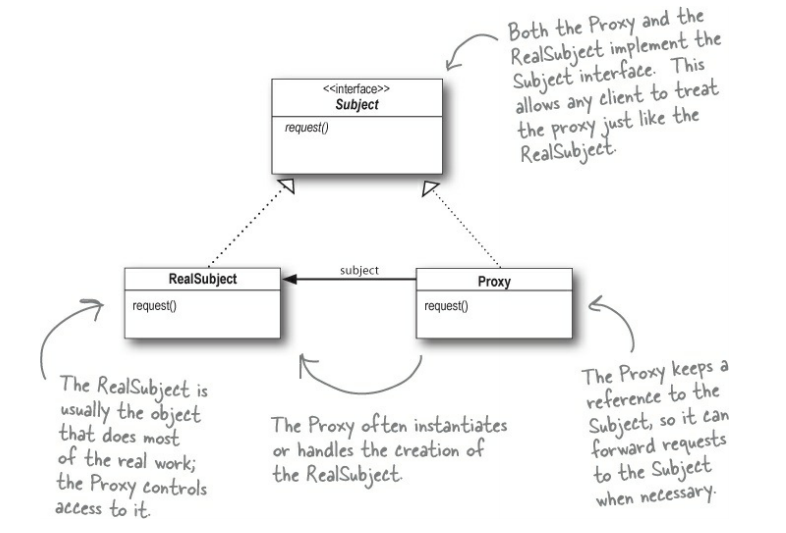
\includegraphics[width=0.5\linewidth]{PatronesSoftware/proxypattern.png}
        \caption{Proxy Pattern}
        \label{fig:proxy-pattern}
\end{figure}

\textbf{Analogía:} Una tarjeta de crédito es un \textbf{proxy} para una cuenta bancaria, la cual es un \textbf{proxy} para un conjunto de dinero en efectivo. Ambas implementan la misma interfaz: pueden usarse para realizar un pago. El consumidor se siente bien porque no necesita llevar grandes cantidades de efectivo. El dueño de la tienda también está contento, ya que el ingreso de una transacción se agrega electrónicamente a la cuenta bancaria de la tienda sin el riesgo de perder el depósito o ser robado en el camino al banco. 

El \textbf{patrón Proxy} puede utilizarse para controlar el acceso a un recurso o servicio, y para realizar autenticación, autorización, registro de actividades (logging) o almacenamiento en caché. Esto puede prevenir accesos no autorizados y ataques de \textbf{inyección SQL}.


\section{Facade Pattern}

El \textbf{patrón Facade} puede utilizarse para proporcionar una interfaz simplificada a un sistema o subsistema complejo, ocultando sus detalles internos y complejidad. Esto puede reducir el acoplamiento y el riesgo de exponer información o funcionalidades sensibles. Puede mejorar la \textbf{modularidad} y \textbf{mantenibilidad} de tu código al separar el subsistema en capas o componentes, así como proteger el subsistema de accesos no autorizados o maliciosos mediante la implementación de verificaciones de seguridad y políticas en la fachada. 

\begin{figure}[H]
    \centering
    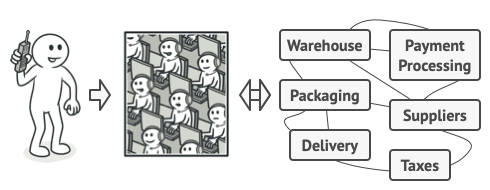
\includegraphics[width=0.5\linewidth]{PatronesSoftware/facade.png}
    \caption{Facade Pattern}
    \label{fig:facade-pattern}
\end{figure}

\textbf{Analogía:} Cuando llamas a una tienda para hacer un pedido por teléfono, un operador actúa como tu \textbf{fachada} ante todos los servicios y departamentos de la tienda. El operador te proporciona una interfaz de voz simple para el sistema de pedidos, las pasarelas de pago y varios servicios de entrega. 

\textbf{Para implementar el patrón Facade}, primero se debe identificar el subsistema que deseas simplificar y asegurar, analizar sus clases, métodos, dependencias e interfaces. Luego, crear una\textbf{ clase fachada }que proporcione una interfaz simple y unificada para el subsistema, con métodos que correspondan a las funcionalidades que los clientes necesitan. Los métodos de la fachada también deben realizar cualquier verificación de seguridad o validación antes de acceder al subsistema. Finalmente, refactoriza los clientes para que utilicen la clase fachada en lugar de interactuar directamente con el subsistema; los clientes solo deben comunicarse con la fachada.

\section{Adapter Pattern}

El \textbf{patrón Adapter} (Adaptador) es un patrón de diseño estructural que permite que dos interfaces incompatibles trabajen juntas. Funciona como un traductor entre dos clases, convirtiendo la interfaz de una clase en otra que el cliente espera, sin cambiar el código existente. Esto podría mejorar la \textbf{interoperabilidad} y \textbf{compatibilidad} de los componentes de tu software, así como prevenir errores o inconsistencias. 

\textbf{Analogía: }Cuando viajas de los EE.UU. a Europa por primera vez, puede que te lleves una sorpresa al intentar cargar tu computadora portátil. Los estándares de los enchufes y tomas de corriente son diferentes en los distintos países. Por eso, tu enchufe de EE.UU. no encajará en una toma de corriente alemana. El problema se puede resolver usando un adaptador de enchufe que tenga el enchufe de estilo americano y la clavija de estilo europeo.

\begin{figure}[H]
    \centering
    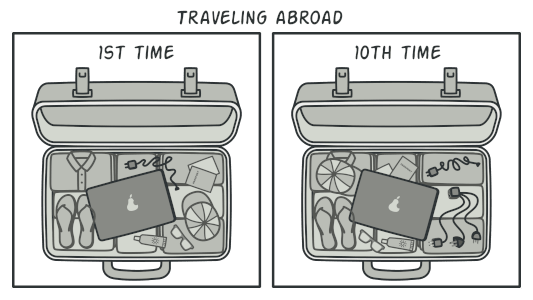
\includegraphics[width=0.5\linewidth]{PatronesSoftware/adapter.png}
    \caption{Adapter Pattern}
    \label{fig:adapter-pattern}
\end{figure}

\textbf{Ejemplo:} Podría usarse un adaptador para traducir las consultas SQL de la aplicación moderna en consultas compatibles con la base de datos antigua, mientras que también implementas medidas de seguridad como parametrización de consultas o escape de caracteres para prevenir SQL Injection. El adaptador actúa como una capa de seguridad entre la base de datos vulnerable y la aplicación moderna, proporcionando una mayor protección sin necesidad de migrar completamente la base de datos.

\section{Singleton}

\textbf{Singleton} es un patrón de diseño creacional que te permite garantizar que una clase tenga solo una instancia, mientras proporciona un punto de acceso global a esta instancia. Puede ayudar a controlar el acceso a recursos sensibles, evitando que partes no autorizadas interfieran con componentes críticos. Ayuda a centralizar las configuraciones relacionadas con la seguridad, asegurando una aplicación consistente de las mismas. 

\begin{figure}[H]
    \centering
    
\includegraphics[width=0.5\linewidth]{PatronesSoftware/singleton.png}
    \caption{Singleton Pattern}
    \label{fig:singleton-pattern}
\end{figure}


\textbf{Analogía: }El gobierno es un excelente ejemplo del patrón Singleton. Un país solo puede tener un gobierno oficial. Independientemente de las identidades personales de las personas que forman los gobiernos, el título 'El Gobierno de X' es un punto de acceso global que identifica al grupo de personas a cargo.

El patrón \textbf{Singleton} puede ser útil cuando se necesita controlar el acceso y el comportamiento de un recurso compartido, como una conexión a la base de datos, un archivo de configuración o un registrador (logger). Uno de los beneficios del patrón Singleton es que puede mejorar la seguridad del sistema al garantizar la consistencia y prevenir el acceso no autorizado o la modificación del recurso compartido. 

Por ejemplo, si se utiliza una clase Singleton para gestionar una conexión a la base de datos, puedes asegurarte de que solo los usuarios autorizados puedan acceder a la base de datos y realizar las operaciones permitidas. También se puede implementar verificaciones de seguridad y mecanismos de registro (logging) en la clase Singleton para monitorear y auditar las actividades en la base de datos. El patrón Singleton también puede prevenir problemas de concurrencia y corrupción de datos al sincronizar el acceso al recurso compartido.


\section{Observer}

El patrón \textbf{Observer} es un patrón de diseño de comportamiento que permite definir un mecanismo de suscripción para notificar a múltiples suscriptores sobre cualquier evento que ocurra en el objeto que están observando. 

\textbf{Analogía: }Si te suscribes a un periódico o revista, ya no necesitas ir a la tienda para ver si el próximo número está disponible. En su lugar, el editor envía los nuevos números directamente a tu buzón tan pronto como se publica, o incluso con antelación. El editor mantiene una lista de suscriptores y sabe a qué revistas están interesados. Los suscriptores pueden salir de la lista en cualquier momento si desean que el editor deje de enviarles los nuevos números de la revista.

\begin{figure}[H]
    \centering
    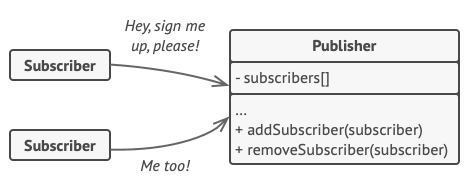
\includegraphics[width=0.5\linewidth]{PatronesSoftware/observer.png}
    \caption{Observer Pattern}
    \label{fig:observer-pattern}
\end{figure}

\textbf{Monitoreo de seguridad en tiempo real:} Imagina que tienes diferentes componentes de seguridad en una red o aplicación, como un sistema de detección de intrusiones (IDS), un firewall, o un antivirus. Usando el patrón \textbf{Observer}, estos sistemas pueden observar eventos importantes que ocurren en el sistema, como accesos no autorizados, intentos de inyección de \ACRshort{sql} o actividad sospechosa. Cuando el sistema principal detecta un evento de seguridad, notifica a todos los observadores (componentes de seguridad) para que tomen las acciones correspondientes (como bloquear una IP, generar una alerta o iniciar un análisis). 

\textbf{Notificación de eventos de seguridad:} En una aplicación o servidor web, podrías tener múltiples observadores que estén pendientes de eventos de seguridad, como la creación de nuevas cuentas de usuario o el acceso a archivos sensibles. Cada vez que ocurre un evento, los observadores pueden recibir una notificación y actuar en consecuencia (alertar a los administradores, registrar la actividad, activar un sistema de defensa, etc.).

\textbf{Autenticación y control de acceso: }En un sistema de control de acceso, podrías tener observadores que vigilan eventos como inicios de sesión fallidos o accesos a recursos sensibles. Si un observador detecta un patrón sospechoso (como demasiados intentos fallidos), puede notificar a otros componentes del sistema para bloquear la cuenta o iniciar un proceso de autenticación más fuerte.

\section{Decorator}

El patrón \textbf{Decorator} es un patrón de diseño estructural que te permite agregar nuevos comportamientos a los objetos colocando estos objetos dentro de objetos envolventes especiales que contienen los comportamientos. A diferencia de la herencia, que altera el comportamiento de un objeto de manera estática, el patrón Decorator ofrece flexibilidad para añadir o quitar comportamientos sobre la marcha sin necesidad de modificar la clase original.

\begin{figure}[H]
    \centering
    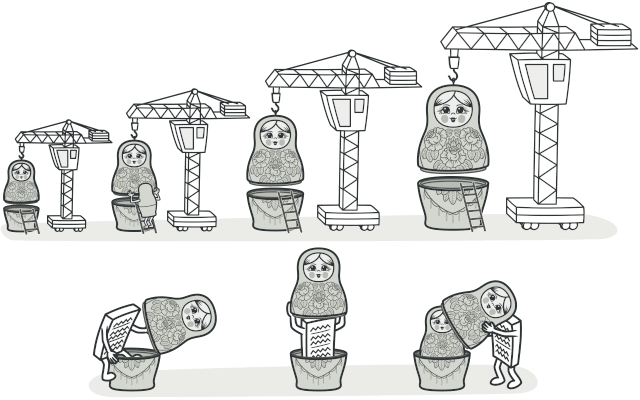
\includegraphics[width=0.5\linewidth]{PatronesSoftware/decorator.png}
    \caption{Decorator Pattern}
    \label{fig:decorator-pattern}
\end{figure}
Analogía: Imagina que tienes un objeto que representa un \textbf{mensaje} en una aplicación. Inicialmente, el mensaje solo tiene la funcionalidad de mostrar texto. Si deseas añadirle características como \textbf{cifrado}, \textbf{compresión}, o \textbf{registro de auditoría} de manera dinámica, puedes envolver el objeto \textbf{mensaje} en varios decoradores que proporcionen estas funcionalidades adicionales sin cambiar la clase original del mensaje. 

El patrón \textbf{Decorator} se puede emplear para agregar capas de seguridad a los objetos de manera dinámica, lo que permite implementar características como \textbf{validación de entradas} y \textbf{codificación de salidas}. Permite la \textbf{adición dinámica de características de seguridad}, adaptándose a las amenazas que evolucionan constantemente.

\section{Strategy}

El patrón \textbf{Strategy} es un patrón de diseño de comportamiento que te permite definir una familia de algoritmos, poner cada uno de ellos en una clase separada y hacer que sus objetos sean intercambiables. Este patrón es útil cuando deseas cambiar el comportamiento de un sistema en tiempo de ejecución, sin modificar el código que usa ese comportamiento.

El patrón \textbf{Strategy} es ideal para \textbf{adaptar algoritmos de seguridad} en función de diferentes tipos de ataques o requisitos de seguridad. Al usar este patrón, puedes implementar múltiples estrategias de seguridad (como cifrado, autenticación, validación, etc.) y elegir cuál usar dependiendo de la situación, sin cambiar la lógica principal del sistema.

\begin{figure}[H]
    \centering
    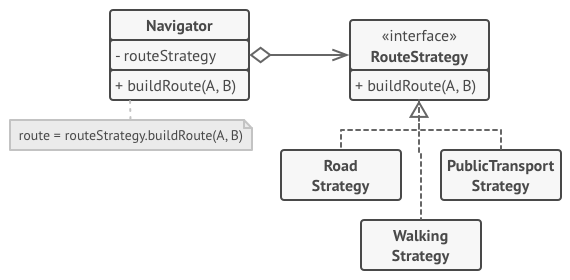
\includegraphics[width=0.5\linewidth]{PatronesSoftware/strategy.png}
    \caption{Strategy Pattern}
    \label{fig:strategy-pattern}
\end{figure}

\textbf{Patrones de diseño y su contribución a la seguridad del software} 

Los patrones de diseño pueden mejorar la seguridad del software al promover el uso de soluciones arquitectónicas probadas y buenas prácticas que mitigan vulnerabilidades comunes. Algunos beneficios clave que los patrones de diseño pueden ofrecer en este ámbito:

\subsubsection{1. \textbf{Encapsulamiento de datos sensibles}}

Los patrones de diseño ayudan a encapsular los datos sensibles, reduciendo el riesgo de vulnerabilidades derivadas de componentes no protegidos o datos inseguros. Patrones como el \textbf{Proxy} permiten acceder a componentes sensibles de manera controlada, previniendo accesos no autorizados.

\subsubsection{2. \textbf{Manejo y prevención de errores}}

Los patrones de diseño también mejoran el manejo de errores y excepciones, evitando que estos se propaguen por la aplicación. Un manejo adecuado de errores es clave para evitar que las vulnerabilidades sean explotadas.

\subsubsection{3. \textbf{Reusabilidad del código}}

Al fomentar la reutilización del código, los patrones de diseño permiten que los desarrolladores utilicen soluciones probadas y seguras, lo que incrementa la robustez del software. El uso de patrones evita la duplicación de código y hace más fácil la aplicación de soluciones de seguridad ya validadas.

\subsubsection{4. \textbf{Mantenibilidad y adaptabilidad}}

Los patrones de diseño promueven la creación de código modular y extensible, facilitando su modificación o extensión sin introducir nuevos riesgos de seguridad. Esto también hace más fácil realizar mejoras o ajustes en la arquitectura de seguridad conforme emergen nuevas amenazas.

\subsubsection{5. \textbf{Pruebas y depuración}}

Al estructurar el código de manera más organizada y modular, los patrones de diseño facilitan las pruebas y la depuración, lo que permite identificar y corregir vulnerabilidades antes de que lleguen a producción. Un código más estructurado es más fácil de probar y asegurar.

\subsubsection{Ventajas generales de los patrones de diseño en seguridad}

Al adherirse a estos patrones de diseño, los desarrolladores establecen una base sólida para las prácticas de codificación segura. Estos patrones no solo ayudan a gestionar la seguridad de manera eficiente, sino que también promueven la mantenibilidad, escalabilidad y resistencia frente a los desafíos de seguridad emergentes.

Sin embargo, Un patrón no es necesariamente una \textbf{mejor práctica} para todos los dominios de problemas o lenguajes, por lo que es importante tratarlos como un conjunto de herramientas, en lugar de soluciones preempaquetadas. Dicho esto, hay \textbf{principios básicos de seguridad} que son esenciales. En particular, nunca confiar en la entrada externa. Siempre se debe sanear los datos de entrada del usuario, realizar validaciones sobre los datos externos, utilizar las características del lenguaje para escapar o parametrizar valores, y escribir pruebas para resultados inválidos al realizar conversiones explícitas de datos en el código.

\chapter{SQL Injection}

\section{Antipatrón}

\subsection*{Nombre}
SQL Injection

\subsection*{También conocido como}
Improper Neutralization of Special Elements used in an SQL Command

\subsection*{Frecuentemente expuesto en el SDLC} 
Diseño

\subsection*{Mapeo con CWE} 
CWE-89

\subsection*{Ejemplos de CVE} 
\begin{itemize}
    \item CVE-2024-7827
    \item CVE-2024-7857
    \item CVE-2011-3130
\end{itemize}

\subsection*{Ejemplo de Anti-patrón}
\begin{itemize}
    \item https://patchstack.com/academy/wordpress/vulnerabilities/sql-injection/
    \item https://cwe.mitre.org/data/definitions/89.html
    
\end{itemize}

\subsection*{Fuerzas desbalanceadas}

\begin{enumerate}
    \item \textbf{Requerimiento de consultas SQL dinámicas: }El sistema permite a los usuarios realizar consultas dinámicas para buscar o filtrar información en la base de datos. Esta flexibilidad responde a la necesidad de ofrecer funcionalidades avanzadas de búsqueda y acceso a los datos. Sin embargo, cuando este requerimiento se implementa sin el uso de parámetros preparados o procedimientos almacenados, y se permite que los datos de entrada del usuario se inserten directamente en la consulta SQL, se expone una vulnerabilidad de inyección SQL. Esto permite que un atacante modifique la semántica de las consultas SQL inyectando código malicioso.
    \item \textbf{Requerimiento de autenticación y autorización:} El sistema permite que los usuarios se autentiquen con credenciales personalizadas, como nombres de usuario y contraseñas, y accedan a sus propios recursos. Este requerimiento es común en sistemas con múltiples roles y privilegios. Sin embargo, si los datos de autenticación se insertan directamente en consultas SQL sin un filtro de validación o escape de caracteres especiales, un atacante podría inyectar comandos SQL maliciosos durante el proceso de inicio de sesión.
\end{enumerate}

\subsection*{Attack pattern}

\begin{itemize}
    \item CAPEC-7
    \item CAPEC-66
    \item CAPEC-108
    \item CAPEC-109
    \item CAPEC-110 
\end{itemize}

\subsection*{Problema}

El sistema no escapa correctamente los caracteres especiales utilizados en la construcción de una consulta SQL, lo que puede alterar el significado de la consulta enviada a la base de datos. Los atacantes pueden inyectar fácilmente su propio código SQL en la consulta ejecutada, lo que permite una amplia variedad de acciones. Por ejemplo, cuando se utilizan consultas SQL en contextos de seguridad, como la autenticación, los atacantes pueden modificar la lógica de esas consultas para obtener acceso no autorizado al ajustar las reglas de autenticación, o eliminando o actualizando registros de la base de datos. 
Los ataques de inyección SQL pueden dirigirse a consultas SQL construidas directamente por el código de la aplicación, o a consultas realizadas por procedimientos almacenados en el cliente o en el servidor. Varios ataques bien conocidos implican comprometer un sistema mediante la inyección de consultas SQL que contienen código malicioso o contenido de la base de datos. 

\subsection*{Consecuancias}

\begin{itemize}
    \item \textbf{Confidencialidad:} Los adversarios podrían ejecutar comandos del sistema, generalmente modificando la declaración SQL para redirigir la salida a un archivo que luego puede ser ejecutado.
    \item \textbf{Autenticación:} Si se utilizan comandos SQL deficientes para verificar nombres de usuario y contraseñas o realizar otros tipos de autenticación, puede ser posible conectarse al producto como otro usuario sin tener conocimiento previo de la contraseña.
    \item \textbf{Control de acceso:} Si la información de autorización se almacena en una base de datos SQL, es posible modificar esta información a través de la explotación exitosa de una vulnerabilidad de inyección SQL.
    \item \textbf{Integridad:} Al igual que es posible leer información sensible, también es posible modificar o incluso eliminar esta información mediante un ataque de inyección SQL.
\end{itemize}

\section{Patrón}

\subsection*{Solucion en el SDLC}

\textbf{Diseño}

\begin{itemize}
    \item Seleccionar una biblioteca o marco de trabajo validado que no permita que esta debilidad ocurra o que proporcione constructos que hagan más fácil evitar esta debilidad. WordPress viene con su propia API de base de datos que proporciona métodos seguros para interactuar con la base de datos. Esta API ayuda a prevenir inyecciones SQL mediante el uso de consultas preparadas y funciones de escape. Otras opciones son PDO (PHP data objects) 
    \item Asegurar el diseño para validar los datos suministrados por los clientes en busca de código malicioso o contenido malformado. Los datos pueden ser basados en formularios, consultas o contenido XML.


\end{itemize}

\textbf{Implementación}

\begin{itemize}
    \item Verificar todas las entradas externas antes de su uso. Utilizar un enfoque de filtros desacoplables y aplicar filtros declarativos basados en URL. Restringir las tareas del filtro para realizar un preprocesamiento de todas las solicitudes y proporcionar validación. Realizar validación del lado del servidor, ya que la validación del lado del cliente no es segura y es susceptible a suplantaciones. Renegociar la confianza entre usuarios después de un intervalo de tiempo específico. Registrar las consultas realizadas e identificar comportamientos irregulares.
    \item La construcción dinámica de consultas se considera generalmente una práctica de desarrollo insegura, pero en algunos contextos, puede ser inevitable. En estos casos, siempre realizar una sanitización cuidadosa de los argumentos de la consulta con un escape correcto de los caracteres especiales dentro de esos argumentos.
\end{itemize}


\subsection*{Ejemplo de Solución}

\begin{itemize}
    \item \href{https://patchstack.com/academy/wordpress/vulnerabilities/sql-injection/}{Patchstack - SQL Injection}
    \item \href{https://cheatsheetseries.owasp.org/cheatsheets/SQL\_Injection\_Prevention\_Cheat\_Sheet.html}{OWASP SQL Injection}
\end{itemize}

\subsection*{Patrones relacionados}

\textbf{Interceptor (POSA)} 

Descripción: Un patrón más general, usado para interceptar y modificar el flujo de ejecución en un sistema antes de que un objeto o componente específico lo procese.
Relación con SQL Injection: Este patrón puede ser implementado para interceptar consultas SQL o solicitudes web y asegurarse de que se sanitizan correctamente antes de ejecutarse en la base de datos.

\textbf{Message Interceptor}

Descripción: Similar al patrón "Intercepting Validator", este patrón intercepta y examina los mensajes de entrada o salida antes de que lleguen a su destino.
Relación con SQL Injection: Permite detectar y eliminar posibles intentos de inyección SQL antes de que los datos sean procesados por la aplicación.

\textbf{Adapt Pattern}

El Adapter Pattern permite adaptar consultas y asegurar la forma en que los datos se envían a la base de datos. En este contexto, el adaptador puede interceptar y transformar las consultas, asegurándose de que los datos están parametrizados y adecuadamente escapados antes de enviarlos a la base de datos. Esto ayuda a evitar que entradas maliciosas del usuario afecten las consultas SQL.


\chapter{Apéndice B: Cross Site Scripting CSS}

\section{Antipatrón}

\subsection{Nombre}
Cross-Site Scripting
\subsection{Tambien conocido como}
Improper Neutralization of Input During Web Page Generation ('Cross-site Scripting')
\subsection{Frecuentemente expuesto en la etapa del SDLC}
Diseño
\subsection{Mapeo con CWE}
CWE-79. 
\subsection{Ejemplos de CVE}
\begin{itemize}
    \item CVE-2024-2194
    \item CVE-2024-5645
    \item CVE-2021-24934
\end{itemize}

\subsection{Ejemplo de antipatrón}

\begin{itemize}
    \item https://patchstack.com/academy/wordpress/vulnerabilities/cross-site-scripting/
    \item https://cwe.mitre.org/data/definitions/79.html
\end{itemize}

\subsection{Fuerzas desbalanceadas}

\begin{itemize}
    \item La ausencia de un requerimiento que para implementar un mecanismo de escape de salida que asegure que todos los datos generados a partir de entradas del usuario sean escapados antes de ser presentados en la interfaz de usuario.
    \item La falta de políticas de validación de entrada que definan qué datos son aceptables y qué formatos deben tener (por ejemplo, validar tipos de datos, rangos y formatos).
    \item La falta de un sistema de filtrado de contenido que procese el HTML proporcionado por el usuario, eliminando o escapando etiquetas y atributos potencialmente peligrosos.
\end{itemize}

\subsection{Attack pattern}
\begin{itemize}
    \item CAPEC-209
    \item CAPEC-588
    \item CAPEC-591
    \item CAPEC-592
    \item CAPEC-63
    \item CAPEC-85
\end{itemize}

\subsection{Problema}

El sistema permite que los usuarios inyecten código malicioso en una página web que será ejecutado por el navegador de otros usuarios. Esto permite a los atacantes robar información sensible, como cookies, o ejecutar acciones en nombre de otros usuarios sin su conocimiento.

\subsection{Consecuencias}

\begin{itemize}
    \item Session Hijacking: Un atacante puede robar la sesión de un usuario.
    \item Defacement: Alteración del contenido visible en la web.
    \item Robo de credenciales: Los atacantes pueden capturar información sensible.
\end{itemize}

\section{Patrón}

\subsection{Solución en el SDLC}
\textbf{Diseño}

\begin{itemize}
    \item Utilizar frameworks y bibliotecas que ofrezcan mecanismos de escape automáticos para prevenir XSS.
    \item Aplicar Content Security Policy (CSP) para reducir la capacidad de ejecutar scripts maliciosos.
    \item Implementar filtros que intercepten y validen todas las entradas de los usuarios.
\end{itemize}

\textbf{Implementación}

\begin{itemize}
    \item Escapar todas las salidas dinámicas de HTML, JavaScript, CSS, PHP, etc.
    \item Verificar y filtrar todas las entradas del usuario en el servidor.
    \item Evitar la construcción dinámica de scripts, y en su lugar utilizar funciones que gestionen el contexto seguro.
\end{itemize}

\subsection{Ejemplo de solución}

\begin{itemize}
    \item \href{https://www.php.net/manual/en/function.htmlspecialchars.php}{PHP Manual}
    \item \href{https://patchstack.com/academy/wordpress/securing-code/cross-site-scripting/}{Patchstack}
    \item \href{https://patchstack.com/academy/wordpress/vulnerabilities/cross-site-scripting/}{Patchstack}
\end{itemize}

\subsection{Patrones relacionados}

\begin{itemize}

    \item \textbf{Decorator Pattern:} Se puede usar un decorador para interceptar y codificar cada comentario antes de que se almacene o se muestre en la página, previniendo que contenido malicioso inyectado pueda ejecutarse en el navegador de otros usuarios. permite aplicar dinámicamente las medidas de seguridad necesarias, como la codificación de salida, en cada lugar donde los datos del usuario se muestren en la interfaz.
    \item \textbf{Sanitizing Input Data:} Limpiar o modificar los datos que provienen de entradas externas para eliminar cualquier contenido malicioso o no deseado, como scripts o código que podría ser usado en ataques.
    La sanitización de entradas asegura que los datos ingresados cumplan con los requisitos del subsistema y de seguridad, eliminando caracteres innecesarios que pueden representar un daño potencial. Desde el navegador del usuario, los datos de entrada viajan a través de solicitudes GET, solicitudes POST y cookies, las cuales los hackers pueden editar, modificar y manipular para obtener acceso al servidor web. La sanitización de entradas actúa como un filtro para depurar los datos codificados a medida que se trasladan al servidor web. Esto se puede hacer de tres maneras:

    \begin{itemize}
        \item White-list sanitization: Permite solo caracteres y cadenas de código válidos.
        \item Black-list sanitization: Limpia la entrada eliminando caracteres no deseados, como saltos de línea, espacios adicionales, tabulaciones, \&, y etiquetas.
        \item Escaping sanitization: Rechaza solicitudes de datos no válidas y elimina las entradas para que no sean interpretadas como código.   
    \end{itemize}
    \item \textbf{Output Encoding} 
    \href{https://docs.oracle.com/en/cloud/saas/marketing/responsys-user/OutputEncodingRequiredFields.html}{Output encoding}

\end{itemize}


\chapter{Apéndice C: Broken Access Control}

\section{Antripatrón}

\subsection{Nombre}
Broken Access Control
\subsection{También conocido como}
Improper Access Control
\subsection{Frecuentemente expuesto en la etapa del SDLC}
Implementación
\subsection{Mapeo con CWE}
CWE-284 (Pillar). Relacionado con:
\begin{itemize}
    \item CWE-862
    \item CWE-863
    \item CWE-732
    \item CWE-306
    \item CWE-1390
    \item CWE-286
    \item CWE-923
\end{itemize}
El control de acceso es un componente crítico en la seguridad de las aplicaciones y sistemas, y abarca varios mecanismos (AAA) claves de protección, entre ellos:

    \begin{itemize}
        \item Autenticación: asegura la identidad del actor que intenta interactuar con el sistema.
        \item Autorización: verifica que el actor autenticado tenga los permisos adecuados para acceder a un recurso o realizar una acción.
        \item Responsabilidad (Accountability): permite rastrear y registrar las actividades que realizan los actores, facilitando auditorías y la detección de comportamientos indebidos.
    \end{itemize}

Dado que el control de acceso cubre múltiples capas de seguridad, cualquier error o debilidad en estos mecanismos puede conducir a vulnerabilidades críticas. Existen numerosas vulnerabilidades registradas en las CWE que están relacionadas con la falta de control de acceso adecuado (BAC). Estas vulnerabilidades pueden variar considerablemente dependiendo de qué aspecto del control de acceso se ataque: desde saltos en la autenticación, hasta escaladas de privilegios o manipulación no autorizada de datos.

A raíz de esto elegí como CWE principal el 284 porque es un pillar. Los \textbf{Pillars }son la categoría más abstracta en el esquema de CWE. Representan los problemas más amplios y conceptuales de seguridad, sin depender de ningún contexto específico de tecnología, software o lenguaje de programación. Los pillars abarcan una gran variedad de debilidades comunes y sirven como la base para organizar problemas de seguridad que podrían surgir en cualquier sistema. Siguiendo el orden de abstracción se encuentran las \textbf{clases} y por último las \textbf{bases}. 

\textbf{Por ej.:} Dentro del pillar CWE-284 se encuentra la clase CWE-285 Improper Authorization. Esta clase describe la vulnerabilidad de productos que no realizan o realizan mal el checkeo de autorización cuando un actor intenta acceder a un recurso. A su vez esta clase es padre de la base CWE-552 que describe la vulnerabilidad de productos como servidores WEB o servidores FPT que no verifican la autorización correctamente, dejando accesible archivos o directorios del sistema.

Para el desarrollo de este VAP, usaré un enfoque general para abarcar todos los tipos de BAC. Los ejemplos serán enfocados a Wordpress.

\subsection{Ejemplos de CVE}

\begin{itemize}
    \item CVE-2023-35093
    \item CVE-2022-45353
    \item CVE-2022-42460
\end{itemize}

\subsection{Ejemplo de antipatrón}

\begin{itemize}
    \item https://patchstack.com/academy/wordpress/vulnerabilities/broken-access-control/
    \item https://owasp.org/Top10/es/A01\_2021-Broken\_Access\_Control/
\end{itemize}

\subsection{Fuerzas desbalanceadas}

\begin{itemize} 
    \item Control de acceso basado en rutas URL: La necesidad de ofrecer acceso a ciertas funcionalidades a través de URL específicas (por ejemplo, /admin, /usuario/{id}) puede llevar a que usuarios no autorizados modifiquen las URL para acceder a recursos restringidos si no se aplica una validación de acceso adecuada en el backend.
    \item Persistencia de sesión en múltiples dispositivos: La necesidad de permitir el acceso a la aplicación desde varios dispositivos y sesiones concurrentes puede llevar a situaciones de control de acceso roto si no se verifican de manera adecuada las sesiones activas y los permisos asociados en cada solicitud.
    \item Control de acceso en API externas: Cuando la aplicación requiere consumir o exponer servicios a través de API, si no se implementan controles de acceso en los endpoints o tokens de autenticación y autorización adecuados, los usuarios pueden acceder a datos o funcionalidades para los que no están autorizados.
\end{itemize}

\subsection{Attack pattern}

\begin{itemize}
    \item CAPEC-284
    \item CAPEC-180
    \item CAPEC-58
    \item CAPEC-122
\end{itemize}


\subsection{Problema}

El sistema permite que los usuarios accedan a funciones o datos que deberían estar restringidos, lo que puede resultar en la exposición de información sensible, modificación de datos, o la realización de acciones no autorizadas. A veces, los desarrolladores realizan la autenticación en el canal principal, pero abren un canal secundario que suponen que es privado. Por ejemplo, un mecanismo de inicio de sesión puede estar escuchando en un puerto de red, pero después de una autenticación exitosa, podría abrir un segundo puerto donde espera la conexión, pero omite la autenticación porque asume que solo la parte autenticada se conectará a ese puerto.

\subsubsection{Consecuencias}
\begin{itemize} 
\item \textbf{Confidencialidad}
Impacto técnico: Leer datos de la aplicación; Leer archivos o directorios.
Un atacante podría leer datos sensibles, ya sea accediendo directamente a una fuente de datos que no esté correctamente restringida, o mediante el acceso a funciones privilegiadas insuficientemente protegidas para leer dichos datos.

\item \textbf{Integridad}
Impacto técnico: Modificar datos de la aplicación; Modificar archivos o directorios.
Un atacante podría modificar datos sensibles, ya sea escribiendo directamente en una fuente de datos que no esté correctamente restringida, o accediendo a funciones privilegiadas insuficientemente protegidas para escribir los datos.

\item \textbf{Control de acceso}
Impacto técnico: Obtener privilegios o asumir identidad; Eludir mecanismos de protección.
Un atacante podría obtener privilegios al modificar o leer datos críticos directamente, o accediendo a funciones privilegiadas.
\end{itemize}

\section{Patrón}

\subsubsection{Solución en el SDLC} \textbf{Diseño} \begin{itemize} \item Implementar controles de acceso desde la etapa de diseño y realizar revisiones de seguridad periódicas. \item Establecer políticas claras de permisos para cada rol de usuario y documentarlas adecuadamente. \item Utilizar técnicas como el principio de menor privilegio para limitar el acceso a recursos sensibles. \end{itemize}

\textbf{Implementación} \begin{itemize} \item Validar los permisos del usuario antes de permitir el acceso a recursos o funciones sensibles. \item No exponer identificadores de recursos directamente en las solicitudes. \item Realizar pruebas de seguridad para identificar y corregir problemas de control de acceso. \end{itemize}

\subsection{Solución}

\begin{itemize}
    \item \href{https://patchstack.com/academy/wordpress/securing-code/broken-access-control/}{Patchstack}
\end{itemize}

\subsection{Related patterns}

\begin{itemize} 
\item \textbf{Proxy Pattern: }Este patrón es ideal para implementar un control de acceso centralizado y eficiente. Al interponer un proxy entre el cliente y los objetos sensibles o restringidos, se puede interceptar cada solicitud y validar los permisos antes de otorgar acceso.
\item \textbf{Decorator: }Este patrón puede ser usado para envolver objetos con capas adicionales de seguridad. Por ejemplo, un decorador podría agregar validaciones de permisos, controles de acceso y logging en tiempo de ejecución, permitiendo reforzar las reglas de acceso y ajustar dinámicamente los controles a nivel de función.
\item \textbf{Input Validation} 
\href{https://cheatsheetseries.owasp.org/cheatsheets/Input_Validation_Cheat_Sheet.html}{OWASP - Input Validation}
\item \textbf{Output Encoding}
\href{https://qwiet.ai/appsec-101-output-encoding/}{Output Encoding}
\item \textbf{Session Management}
\href{https://cheatsheetseries.owasp.org/cheatsheets/Session_Management_Cheat_Sheet.html}{Session Management}
\end{itemize}

\chapter{Cross-Site Request Forgery}
\section{Antipatrón}
\subsection{Nombre} 
Cross-Site Request Forgery

\subsection{También conocido como} 
Sea Surf, Session Riding, XSRF

\subsection{Frecuentemente expuesto en la etapa del SDLC} 
Requerimientos, Implementación

\subsection{Mapeo con CWE} \textbf{CWE-352 (Composite)}. Al ser un composite, CSRF es la combinación de varias vulnerabilidades explotadas. Estas son: 
\begin{itemize}
    \item \textbf{CWE-346: Origin Validation Error} – Fallas en la validación del origen de las solicitudes (por ejemplo, falta de verificación de los encabezados de origen o referer), lo que facilita ataques de CSRF.
    \item \textbf{CWE-441: Unintended Proxy or Intermediary (Confused Deputy)} – Describe escenarios en los que un servidor o aplicación actúa como un proxy involuntario para un atacante, lo que puede ocurrir en situaciones de CSRF.
    \item \textbf{CWE-642: External Control of Critical State Data} – En el contexto de CSRF, se refiere a la manipulación o control externo de datos críticos de estado, como tokens de autenticación o cookies de sesión.
    \item \textbf{CWE-613: Insufficient Session Expiration} – Se refiere a la incapacidad para terminar una sesión correctamente, lo que permite a un atacante reutilizar sesiones o explotar vulnerabilidades como CSRF durante una sesión activa.
\end{itemize}
\subsection{Ejemplos de CVE}
\begin{itemize}
    \item CVE-2024-44028
    \item CVE-2024-43301
    \item CVE-2023-27634
\end{itemize}

\subsection{Ejemplo de antipatrón} 

\begin{itemize}
    \item \href{https://patchstack.com/academy/wordpress/vulnerabilities/cross-site-request-forgery/}{Patchstack}
    \item \href{https://cwe.mitre.org/data/definitions/352.html}{CWE}
\end{itemize}

\subsection{Fuerzas desbalanceadas} \begin{itemize} \item Uso de cookies para autenticación \item Uso de la misma sesión en múltiples pestañas o ventanas. \item No validar correctamente las solicitudes del usuario con un token CSRF \item Múltiples aplicaciones alojadas en un mismo dominio. Las cookies (que se usan para mantener la sesión del usuario) pueden ser compartidas entre subdominios. Esto se debe a que las políticas de mismo origen (Same-Origin Policy) que suelen proteger las solicitudes AJAX no siempre se aplican a las cookies. \end{itemize}

\subsection{Attack pattern} 
\begin{itemize}
    \item CAPEC-111
    \item CAPEC-462
    \item CAPEC-467
    \item CAPEC-62
\end{itemize}

\subsection{Problema} Un atacante puede enviar una solicitud maliciosa que se ejecutará bajo la credencial de un usuario autenticado, realizando acciones que el usuario no tenía intención de realizar, como cambiar su configuración, hacer transacciones o realizar acciones administrativas.

\subsection{Consecuencias} 

\textbf{Confidencialidad:} Impacto Técnico: Obtener privilegios o asumir la identidad; Eludir el mecanismo de protección; Leer datos de la aplicación; Modificar datos de la aplicación; Denegación de servicio: Bloqueo, Cierre o Reinicio. 

\textbf{Integridad, Disponibilidad, No Repudio, Control de Acceso: }Las consecuencias variarán según la naturaleza de la funcionalidad que sea vulnerable a CSRF. Un atacante podría realizar cualquier operación como si fuera la víctima. Si la víctima es un administrador o un usuario con privilegios, las consecuencias pueden incluir obtener control total sobre la aplicación web: eliminar o robar datos, desinstalar el producto o utilizarlo para lanzar otros ataques contra todos los usuarios del producto. Debido a que el atacante asume la identidad de la víctima, \textbf{el alcance del ataque CSRF solo está limitado por los privilegios de la víctima. }

\section{Patrón}

\subsubsection{Solución en el SDLC} \textbf{Diseño:} \begin{itemize} \item Incluir la generación y verificación de tokens únicos por usuario para cada solicitud (tokens anti-CSRF). \item Implementar controles adicionales, como la verificación del encabezado Referer o Origin para asegurar que las solicitudes provengan de fuentes confiables. \end{itemize}

\textbf{Implementación:} \begin{itemize} \item Incluir un token anti-CSRF en cada formulario o solicitud sensible y validarlo en el lado del servidor. \item Asegurarse de que los formularios importantes y solicitudes sensibles se envíen solo por métodos HTTP POST y no GET. \item Utilizar técnicas como SameSite para las cookies, reduciendo la exposición a CSRF. \end{itemize}

\subsection{Soluciones}

\begin{itemize}
    \item \href{https://patchstack.com/academy/wordpress/securing-code/cross-site-request-forgery/}{Patchstack}
    \item \href{https://cheatsheetseries.owasp.org/cheatsheets/Cross-Site_Request_Forgery_Prevention_Cheat_Sheet.html}{OWASP}
\end{itemize}

\subsection{Patrones relacionados}

\begin{itemize}
    \item Uso de tokens anti-CSRF en aplicaciones web. Este patrón de seguridad incluye generar un token único para cada sesión de usuario y adjuntarlo a solicitudes críticas que involucran cambios de estado.
    \item Utilizar patrones como el \textbf{Synchronizer Token Pattern} para asegurar que solo las solicitudes legítimas sean procesadas. Cada solicitud debe incluir un token único que se valida en el servidor. El STP se utiliza cuando el usuario solicita una página con datos de un formulario:
    \begin{enumerate}
        \item El servidor envía un token asociado con la identidad actual del usuario al cliente.
        \item El cliente envía de vuelta el token al servidor para su verificación.
        \item Si el servidor recibe un token que no coincide con la identidad del usuario autenticado, la solicitud es rechazada.
    \end{enumerate}
\end{itemize}




\chapter{Apéndice D: Server Side Request Forgery}
\section{Antipatrón}
\subsection{Nombre}
Server Side Request Forgery
\subsection{Tambien conocido como}
SSRF
Cross Site Port Attack
\subsection{Frecuentemente expuesto en la etapa del SDLC}
Diseño
Implementación
\subsection{Mapeo con CWE}
CWE-918
\subsection{Ejemplos de CVE}
\begin{itemize}
    \item CVE-2024-43989
    \item CVE-2024-5021
\end{itemize}
\subsection{Ejemplo de antipatrón}

\begin{itemize}
    \item \href{https://patchstack.com/academy/wordpress/vulnerabilities/server-side-request-forgery/}{Patchstack}
    \item \href{https://cwe.mitre.org/data/definitions/918.html}{CWE}
\end{itemize}

\subsection{Fuerzas desbalanceadas}

\begin{itemize}
    \item La aplicación permite a los usuarios interactuar con recursos externos, como la descarga de archivos o la obtención de información. Esta flexibilidad genera una vulnerabilidad cuando se implementa sin restricciones de validación en las URLs externas que los usuarios pueden enviar.
    \item La implementación que permite que los usuarios envíen solicitudes sin validación hace que el servidor actúe como una "ventana" hacia su propia red interna. Un atacante puede aprovechar esto para acceder a recursos internos que normalmente no están disponibles desde el exterior, como por ejemplo una base de datos. 
\end{itemize}

\subsection{Attack pattern}
CAPEC-664
\subsection{Problema}

El servidor web recibe una URL o una solicitud similar de un componente aguas arriba y recupera el contenido de esa URL, pero no garantiza suficientemente que la solicitud se esté enviando al destino esperado.
Al proporcionar URLs a hosts o puertos inesperados, los atacantes pueden hacer que parezca que el servidor está enviando la solicitud, lo que posiblemente permite eludir controles de acceso, como cortafuegos que impiden que los atacantes accedan directamente a las URLs. El servidor puede ser utilizado como un proxy para realizar escaneos de puertos en hosts de redes internas, usar otras URLs que puedan acceder a documentos en el sistema (usando file://), o utilizar otros protocolos como gopher:// o tftp://, los cuales pueden ofrecer un mayor control sobre el contenido de las solicitudes.

\subsection{Consecuencias}

Confidencialidad: lectura de datos sensibles de la aplicación

Integridad: modificar datos o realizar acciones no autorizadas dentro de la infraestructura interna.

\section{Patrón}
\subsubsection{Solución en el SDLC}
Diseño
\begin{itemize}
    \item Restringir el uso de protocolos innecesarios como file://, gopher://, o schema://. Un atacante puede usarlos para evadir las restricciones que has establecido.
    \item Aplicar el principio de privilegios minimos que establece que un usuario solo debe recibir los derechos mínimos necesarios para realizar una operación, y solo por el tiempo estrictamente necesario.

\end{itemize}
Implementación
\begin{itemize}
    \item Usa siempre mensajes de error genéricos y no verbosos. Un actor malicioso podría usar mensajes verbosos para realizar ataques a ciegas.
    \item Validar y sanitizar correctamente la entrada proporcionada por el usuario antes de pasarla a métodos sensibles como los analizadores de URL. Considera la entrada del usuario como no confiable al escribir código.
    \item Usar validación basada en una lista de permitidos (allowlist) para las direcciones IP y nombres DNS a los que tu aplicación necesita acceder. Esto previene que un atacante intente solicitar recursos no previstos.
    \item Usar un firewall para aplicaciones web (WAF) con reglas de bloqueo estrictas para detectar, bloquear y registrar cualquier carga maliciosa o entrada no deseada.
    \item Usar las funciones de seguridad que ofrece tu proveedor de la nube para mitigar vulnerabilidades comunes. Por ejemplo, AWS Cloud ofrece el método de Instance Metadata Service Version 2 (IMDSv2) que protege contra ataques SSRF y bloquea el acceso no autorizado a metadatos.
    
\end{itemize}
\subsection{Ejemplo de solución}

\begin{itemize}
    \item \href{https://patchstack.com/academy/wordpress/securing-code/server-side-request-forgery/}{PatchStack}
\end{itemize}

\subsection{Related patterns}

\textbf{Proxy Pattern} 

Permite controlar y filtrar las solicitudes realizadas desde el servidor hacia recursos externos, lo cual es clave para mitigar el riesgo de SSRF. Proporciona una capa de control que permite filtrar, validar, y registrar las solicitudes salientes.

\textbf{Funciones de Wordpress} 

Si el plugin o tema necesita obtener o realizar una solicitud a una URL externa, podemos usar las funciones integradas de WordPress dependiendo de los métodos HTTP, como: 

\begin{itemize}
    \item wp\_safe\_remote\_head
    \item wp\_safe\_remote\_get
    \item wp\_safe\_remote\_post
    \item wp\_safe\_remote\_request
\end{itemize}

Las funciones anteriores protegerán principalmente contra la vulnerabilidad SSRF y negarán el acceso a un servicio interno. Sin embargo, ten en cuenta que actualmente las funciones anteriores no son 100% seguras y existen algunos casos raros que aún permiten el acceso a servicios internos. Por favor, consulta este artículo:

\href{https://patchstack.com/articles/exploring-the-unpatched-wordpress-ssrf/}{Explorando lo desconocido: debajo de la superficie de la vulnerabilidad SSRF sin parche en WordPress} 

\textbf{Saneamiento y Validación} 

Como ocurre con la mayoría de las vulnerabilidades, un punto crítico en los ataques SSRF es el uso de datos no confiables. Siempre debe tratarse cualquier dato que provenga del lado del cliente como no confiable.

Saneando y validando los datos proporcionados por el cliente se puede avanzar mucho en la defensa contra ataques SSRF. Una validación muy intuitiva es restringir cualquier URL que contenga "localhost" o la dirección de loopback.



\chapter{Path Traversal}

\section{Antipatrón}

\subsection*{Nombre}
Path Traversal

\subsection*{También conocido como}
\begin{itemize}
    \item Directory Traversal
    \item Path Traversal Attack
\end{itemize}

\subsection*{Frecuentemente expuesto en la etapa del SDLC}

Diseño, Implementación.

\subsection*{Mapping con CWE}
CWE-22: Improper Limitation of a Pathname to a Restricted Directory ('Path Traversal')

\subsection*{Ejemplos de CVE}
CVE-2024-0221
CVE-2024-9047

\subsection*{Ejemplo del Antipatrón}

\begin{itemize}
    \item \href{https://cwe.mitre.org/data/definitions/22.html}{CWE}
    \item \href{https://owasp.org/www-community/attacks/Path_Traversal}{OWASP}
\end{itemize}

\subsection*{Fuerzas desbalanceadas}

1. Entrada del usuario no restringida: La necesidad de ofrecer al usuario la opción de cargar archivos o acceder a recursos externos puede derivar en la manipulación de rutas si no se realiza una validación adecuada.
2. Acceso directo a archivos del servidor: El sistema permite acceder a archivos del servidor en función de entradas proporcionadas por el usuario, lo que puede llevar a la exposición de archivos sensibles si no se controla adecuadamente la ruta solicitada.

\subsection*{Attack Pattern}
CAPEC-126: Path Traversal

\subsection*{Problema}

El producto utiliza una entrada externa para construir una ruta que tiene la intención de identificar un archivo o directorio ubicado debajo de un directorio padre restringido, pero el producto no neutraliza adecuadamente los elementos especiales dentro de la ruta que pueden hacer que la ruta se resuelva en una ubicación fuera del directorio restringido.

Muchas operaciones de archivos están destinadas a realizarse dentro de un directorio restringido. Al usar elementos especiales como ".." y los separadores de "/", los atacantes pueden escapar de la ubicación restringida para acceder a archivos o directorios que se encuentran en otra parte del sistema. Uno de los elementos especiales más comunes es la secuencia "../", que en la mayoría de los sistemas operativos modernos se interpreta como el directorio padre de la ubicación actual. Esto se conoce como traversal relativo de ruta.

El traversal de ruta también abarca el uso de nombres de ruta absolutos como \href{usr/local/bin} para acceder a archivos inesperados. Esto se conoce como traversal absoluto de ruta. 

\subsection*{\textbf{Consecuencia}}

1. Integridad: El atacante podría ser capaz de sobrescribir o crear archivos críticos, como programas, bibliotecas o datos importantes. Si el archivo objetivo es utilizado por un mecanismo de seguridad, el atacante podría eludir ese mecanismo. Por ejemplo, agregar una nueva cuenta al final de un archivo de contraseñas podría permitir a un atacante eludir la autenticación.

2. Conficencialidad: El atacante podría ser capaz de leer el contenido de archivos inesperados y exponer datos sensibles. Si el archivo objetivo es utilizado por un mecanismo de seguridad, el atacante podría eludir ese mecanismo. Por ejemplo, al leer un archivo de contraseñas, el atacante podría realizar ataques de fuerza bruta para intentar adivinar las contraseñas y acceder a una cuenta en el sistema.

3. Disponibilidad: El atacante podría ser capaz de sobrescribir, eliminar o corromper archivos críticos inesperados, como programas, bibliotecas o datos importantes. Esto podría impedir que el producto funcione correctamente y, en el caso de mecanismos de protección como la autenticación, tiene el potencial de bloquear a los usuarios del producto.


\section{Patrón}

\subsection*{Pasos de la solución en el SDLC}

\textbf{Diseño:}

\begin{itemize}
    \item Configurar correctamente el control de acceso.
    \item Hacer cumplir el principio de privilegios mínimos.
    \item Ejecutar programas con privilegios restringidos, de manera que el proceso padre no abra más vulnerabilidades. Asegúrate de que todos los directorios, archivos temporales y de memoria se ejecuten con privilegios limitados para proteger contra la ejecución remota.
    \item Validación de entradas. Asumir que las entradas del usuario son maliciosas. Utilizar un estricto control de tipos, caracteres y codificación.
    \item Comunicación proxy al host, de modo que las comunicaciones se terminen en el proxy, sanitizando las solicitudes antes de enviarlas al servidor.
    \item Ejecutar interfaces de servidor con una cuenta no-root y/o utilizar jaulas chroot u otras técnicas de configuración para restringir privilegios, incluso si un atacante obtiene acceso limitado a los comandos.
\end{itemize}

\textbf{Implementación:}

\begin{itemize}
    \item Monitoreo de la integridad del host para archivos, directorios y procesos críticos. El objetivo es estar al tanto cuando ocurra un problema de seguridad para que se inicien actividades de respuesta a incidentes y forenses.
    \item Realizar validación de entrada para todo el contenido remoto, incluyendo contenido remoto y generado por usuarios.
    \item Realizar pruebas como pen-testing y escaneo de vulnerabilidades para identificar directorios, programas e interfaces que otorgan acceso directo a ejecutables.
    \item Usar referencias indirectas en lugar de nombres de archivos reales.
    \item Utilizar los permisos posibles en el acceso a archivos al desarrollar y desplegar aplicaciones web.
    \item Validar la entrada del usuario solo aceptando datos conocidos como válidos. Asegurarse de que todo el contenido entregado al cliente esté sanitizado de acuerdo a una especificación de contenido aceptable, utilizando un enfoque de lista blanca.
\end{itemize}

\subsection*{\textbf{Solución}}

\href{https://www.wpservices.com/stay-secure-protecting-your-wordpress-site-from-directory-traversal-vulnerabilities/}{WPServicses}

\href{https://patchstack.com/academy/wordpress/securing-code/arbitrary-file-deletion/#how-to-secure}{PatchStack - File Deletion}

\href{https://patchstack.com/academy/wordpress/securing-code/arbitrary-file-read/#how-to-secure}{PatchStack - FIle Read}

\href{https://patchstack.com/academy/wordpress/securing-code/arbitrary-file-deletion/}{PatchStack - File Deletion}

\textbf{Patrones relacionados}

\begin{itemize}
    \item Facade Pattern: puede proporcionar una interfaz simplificada y controlada para el acceso a recursos del sistema de archivos, permitiendo que las rutas de archivo sean verificadas y sanitizadas antes de que se realicen las operaciones de lectura o escritura. 
    \item Funcionalidades de WordPress: utilizar funciones para sanitizar la entrada como \path{esc\_url()} y \path{esc\_url\_raw()}.
    \item Deshabilitar indexado de directorios: modificando las reglas de .htaccess se puede prevenir que los atacantes enumeren el contenido de los directorios  e identifiquen posibles puntos de ataque.
\end{itemize}


\chapter{Remote/Local File Inclusion}

Estas dos vulnerabilidades se detallan juntas ya que la única diferencia entre ellas es el origen desde el cual el atacante incluye un archivo en el servidor. Puede ser archivos locales o un archivo remoto del servidor del atacante. 

\section{Antipatrón}
\subsection*{Nombre}
Remote/Local File Inclusion
\subsection*{Tambien conocido como}
\begin{itemize}
    \item Remote file include
    \item RFI
    \item Local file inclusion
\end{itemize}
\subsection*{Frecuentemente expuesto en la etapa del SDLC}
Implementación
\subsection*{Mapeo con CWE}
CWE-98
\subsection*{Ejemplos de CVE}
CVE-2024-34551 
CVE-2024-49286 
CVE-2024-44014 
\subsection*{Ejemplo de antipatrón}

\begin{itemize}
    \item https://cwe.mitre.org/data/definitions/98.html
    \item https://patchstack.com/academy/wordpress/vulnerabilities/local-file-inclusion/
\end{itemize}


\subsection*{Fuerzas desbalanceadas}

\begin{itemize}
    \item El sistema permite la inclusión de archivos mediante rutas proporcionadas por el usuario pero estas no se validan correctamente permitiendo al atacante incluir archivos locales (LFI) o remotos (RFI).
    \item El sistema permite la inclusión de archivos especificados por el usuario pero estas no se validan correctamente, permitiendo a un atacante ejecutar un archivo local sensible.
\end{itemize}

\subsection*{Attack pattern}

CAPEC-193
CAPEC-252

\subsection*{Problema}
La aplicación PHP permite que el atacante controle qué archivo será incluido o requerido mediante funciones como require, include, include\_once, o require\_once. El problema clave es que la aplicación no valida ni restringe correctamente la entrada del usuario, lo que puede permitir la ejecución de código malicioso o la exposición de información sensible.
\subsection*{Consecuencias}
\textbf{Integridad, confidencialidad y disponibilidad:} El atacante puede especificar código arbitrario que será ejecutado desde una ubicación remota. Alternativamente, puede ser posible aprovechar el comportamiento normal del programa para insertar código PHP en archivos en la máquina local, los cuales luego pueden ser incluidos, forzando así la ejecución del código, ya que PHP ignora todo en el archivo excepto el contenido entre los delimitadores de PHP.

\section{Patrón}

\subsection*{Solución en el SDLC}

Implementación:

\begin{itemize}
    \item Whitelist de archivos: Crear una lista blanca de archivos que pueden ser incluidos y nunca permitir la inclusión arbitraria.
    \item Forzar el uso de rutas absolutas y nunca confiar en entradas directas del usuario.
    \item Utiliza referencias indirectas pasadas en los parámetros de la URL en lugar de nombres de archivos, por ej.: \textit{https://example.com/view?file\_id=123} donde \textit{file\_id=123} no es directamente un archivo, sino un identificador interno. El servidor resuelve ese identificador en un archivo permitido, previniendo el acceso a rutas no autorizadas.
    \item Usar configuraciones de PHP para limitar la superficie de ataque. Desactivar la opcion allow\_url\_fopen que limita la habilidad de incluir archivos en ubicaciones remotas.
\end{itemize}

\subsection*{Solución}

\begin{itemize}
    \item \href{https://owasp.org/www-project-web-security-testing-guide/v42/4-Web_Application_Security_Testing/07-Input_Validation_Testing/11.2-Testing_for_Remote_File_Inclusion}{OWASP Web Security Testing Guide}
    \item \href{https://patchstack.com/academy/wordpress/securing-code/local-file-inclusion/}{PatchStack - Local File Inclusion}
\end{itemize}

\subsection*{Patrones relacionados}

\begin{itemize}
    \item \textbf{Adapter Pattern:} Si una aplicación necesita interactuar con bases de datos o archivos locales,  un adaptador puede actuar como una capa de seguridad para asegurar que las consultas estén parametrizadas y que los inputs se saniticen antes de procesarlos. Por ejemplo, podriamos utilizar un adaptador para implementar referencias indirectas a archivos del servidor.
    \item Utilizar versiones recientes de PHP (preferiblemente PHP 6 o posterior, aunque hoy en día ya estamos en versiones PHP 7.x y 8.x). Las versiones más recientes de PHP incluyen mejoras significativas de seguridad que no estaban presentes en las versiones anteriores (especialmente las versiones de PHP 4.x o 5.x). Muchas vulnerabilidades y prácticas inseguras que existían en versiones antiguas han sido corregidas o eliminadas en versiones modernas
    \item Utilizar un WAF como medida temporal mientras se desarrollan parches o actualizaciones para corregir las vulnerabilidades en el código.
    \item Almacena las bibliotecas, archivos de inclusión y archivos de utilidad fuera del directorio raíz de documentos web, si es posible y utilizar las configuraciones del servidor web para restringir el acceso directo a estos archivos.
\end{itemize}






\chapter{Remote Code Execution}
\section{Antipatrón}
\subsection*{Nombre}
Remote Code Execution.
\subsection*{Tambien conocido como}
Code Injection. 
\subsection*{Frecuentemente expuesto en la etapa del SDLC}
Implementación.
\subsection*{Mapeo con CWE}
CWE-94
\subsection*{Ejemplos de CVE}
CVE-2024-50498
CVE-2024-25600
CVE-2006-2667
\subsection*{Ejemplo de antipatrón}
\begin{itemize}
    \item https://www.invicti.com/learn/remote-code-execution-rce/
    \item https://patchstack.com/academy/wordpress/vulnerabilities/remote-code-execution/
    \item https://cwe.mitre.org/data/definitions/94.html
\end{itemize}
\subsection*{Fuerzas desbalanceadas}
\begin{itemize}
    \item Cuando un producto permite que la entrada del usuario contenga sintaxis de código, es posible que un atacante pueda manipular ese código de tal manera que altere el flujo de control previsto del producto. Dicha alteración podría llevar a la ejecución de código arbitrario.
    \item El producto construye todo o parte de un segmento de código utilizando entradas influenciadas externamente desde un componente ascendente, pero no neutraliza o neutraliza incorrectamente elementos especiales que podrían modificar la sintaxis o el comportamiento del segmento de código previsto.
\end{itemize}
\subsection*{Attack pattern}
CAPEC-242
\subsection*{Problema}
RCE permite que un atacante ejecute comandos o código arbitrario en el servidor. Esto ocurre por errores en la validación y sanitización de entradas, o en el uso inseguro de funciones críticas de ejecución.
\subsection*{Consecuencias}
\begin{itemize}
    \item Control de acceso: En algunos casos, el código inyectable controla la autenticación; esto puede conducir a una vulnerabilidad remota. El código inyectado puede acceder a recursos a los que el atacante no puede acceder directamente.
    \item Integridad, confidencialidad y disponibilidad: Al inyectar código malicioso en el plano de control, un atacante puede alterar la forma en que el sistema interpreta y ejecuta las órdenes, lo que le permite realizar acciones no autorizadas. En algunos casos, los ataques de inyección de código pueden permitir a un atacante obtener acceso a partes del sistema con mayores privilegios, como la base de datos o el sistema operativo. 
\end{itemize}

\section{Patrón}

\subsection*{Solución en el SDLC}

\textbf{Implementación}

\begin{itemize}
    \item Asumir que toda entrada es maliciosa: Tratar todos los datos de entrada como si fueran potencialmente dañinos.
    \item Utiliza una estrategia de validación de entrada "acepta lo conocido como bueno": Define una lista estricta de entradas válidas y rechaza cualquier entrada que no cumpla con estos criterios o transformala en una entrada válida.
    \item Validar todas las propiedades relevantes: Considerar la longitud, el tipo de entrada, el rango de valores aceptables, entradas faltantes o adicionales, la sintaxis, la consistencia entre campos relacionados y la conformidad con las reglas de negocio.
    \item No confíar únicamente en la detección de entradas maliciosas o malformadas: Esto puede dejar pasar entradas no deseadas, especialmente si el entorno del código cambia. Usa listas negras para detectar posibles ataques o rechazar entradas extremadamente malformadas.
\end{itemize}

\subsection*{Ejemplo de solución}

\begin{itemize}
    \item https://patchstack.com/academy/wordpress/securing-code/remote-code-execution/
\end{itemize}

\subsection*{Related patterns}

\begin{itemize}
    \item Proxy Pattern: Al actuar como intermediario, el Proxy puede filtrar y validar todas las solicitudes antes de llegar al objeto real. Esto permite implementar mecanismos de autorización y autenticación robustos, evitando que código malicioso se ejecute.
    \item Sanitizar entradas: Validar y limpiar los datos proporcionados por el usuario antes de utilizarlos en la aplicación. Esto incluye verificar tipos de datos, longitudes, formatos y utilizar listas blancas para restringir los valores permitidos.
    \item Gestión de memoria: Los desbordamientos de búfer son una causa común de RCE. Utilizar técnicas de asignación y liberación de memoria seguras, realizar análisis de vulnerabilidad de forma regular y aplicar parches a las vulnerabilidades encontradas.
\end{itemize}


\chapter{CSV Injection}
\section{Antipatrón}
\subsection{Nombre}
 CSV Injection 
\subsection{Tambien conocido como}
Formula Injection. Excel Macro Injection	
\subsection{Frecuentemente expuesto en la etapa del SDLC}
Implementación
\subsection{Mapeo con CWE}
CWE-1236
\subsection{Ejemplos de CVE}
CVE-2022-46821

\subsection{Ejemplo de antipatrón}
\begin{itemize}
    \item https://cwe.mitre.org/data/definitions/1236.html
\end{itemize}
\subsection{Fuerzas desbalanceadas}
\begin{itemize}
    \item El requerimiento de exportar datos de usuario en formato CSV para su descarga y análisis lleva a la exposición a vulnerabilidades de CSV Injection si no se implementa una sanitización adecuada de los datos exportados.
    \item El requerimiento de generar reportes (o cualquier tipo de contenido representable en CSV) en formato CSV con datos generados dinámicamente por el usuario lleva a la exposición a CSV Injection si  los valores dinámicos no son controlados.
\end{itemize}
\subsection{Attack pattern}
CAPEC-23
\subsection{Problema}
CSV Injection ocurre cuando datos sin sanitizar se exportan en formato CSV y luego son abiertos en aplicaciones que ejecutan automáticamente fórmulas o scripts. Esto puede permitir que se ejecute código en el sistema del usuario al abrir el archivo.
\subsection{Consecuencias}
Confidencialidad: los .csv maliciosamente elaborados pueden ser utilizados para tres ataques clave:
\begin{itemize}
    \item Secuestrar la computadora del usuario explotando vulnerabilidades en el software de hojas de cálculo.
    \item Secuestrar la computadora del usuario explotando la tendencia del usuario a ignorar las advertencias de seguridad en hojas de cálculo que descargaron del sitio web.
    \item Exfiltrar contenido de la hoja de cálculo, o de otras hojas de cálculo abiertas."
\end{itemize}


\section{Patrón}
\subsection{Solución en el SDLC}
Implementación: Sanitizar cualquier dato que se exporta en formato CSV, prefijando caracteres peligrosos como =, +, -, o @ con un apóstrofo (') para prevenir la ejecución como fórmula.
\subsection{Ejemplo de solución}
\begin{itemize}
    \item https://www.cyberchief.ai/2024/09/csv-formula-injection-attacks.html
    \item https://owasp.org/www-community/attacks/CSV\_Injection
    \item https://patchstack.com/articles/patchstack-weekly-what-is-csv-injection
\end{itemize}
\subsection{Related patterns}
\begin{itemize}
    \item Sanitizar entradas
    \item Codificación y escapado de datos
    \item Facade: Este patrón puede ser implementado para agrupar las tareas relacionadas con la creación de archivos CSV, como la validación de las entradas, la sanitización de los datos (por ejemplo, para evitar la ejecución de fórmulas), y luego generar el archivo CSV de forma segura.
\end{itemize}

\chapter{Data Exposure}
\section{Antipatrón}
\subsection{Nombre}
Data exposure
\subsection{Tambien conocido como}
Exposure of Sensitive Information to an Unauthorized Actor
Information Disclosure
Information Leak
\subsection{Frecuentemente expuesto en la etapa del SDLC}
Arquitectura
Implementación
\subsection{Mapeo con CWE}
CWE-200
\subsection{Ejemplos de CVE}
CVE-2024-10285
CVE-2024-2107
CVE-2013-2203 
\subsection{Ejemplo de antipatrón}
https://cwe.mitre.org/data/definitions/200.html
\subsection{Fuerzas desbalanceadas}
\begin{itemize}
    \item Un sistema de login con usuario y clave que avisa al usuario de que colocó una contraseña incorrecta, está revelando información sobre la existencia de ese usuario, lo que puede facilitar ataques de fuerza bruta.
    \item El código gestiona recursos que contienen intencionalmente información sensible, pero estos recursos se hacen accesibles de forma no intencionada para actores no autorizados. 
    \item La manipulación de datos sensibles de usuario sin el cifrado correcto durante su transmisión o almacenamiento, podrían ser interceptados o accesibles a personas no autorizadas. 
    \item El sistema permite un acceso uniforme a todos los usuarios sin una estructura de roles por detrás lo que puede dar acceso a datos sensibles a usuarios no autorizados.
\end{itemize}
\subsection{Attack pattern}
CAPEC-116
\subsection{Problema}
El producto expone información sensible a un actor que no está explícitamente autorizado para acceder a esa información. Las exposiciones de información pueden ocurrir de diversas maneras:
    \begin{itemize}
        \item El código inserta explícitamente información sensible en recursos o mensajes que son intencionalmente accesibles para actores no autorizados, pero que no deberían contener dicha información; es decir, la información debería haber sido "limpiada" o "saneada".
        \item Una debilidad o error diferente (podria ser un plugin o tema vulnerable) inserta indirectamente la información sensible en los recursos, como un error en un script web que revela la ruta completa del sistema donde se encuentra el programa.
        \item El código gestiona recursos que contienen intencionalmente información sensible, pero estos recursos se hacen accesibles por error a actores no autorizados. En este caso, la exposición de la información es resultante; es decir, una debilidad diferente permitió el acceso a la información desde el inicio.
    \end{itemize}
\subsection{Consecuencias}
Confidencialidad:
\begin{itemize}
    \item Exposición de datos personales o privados, afectando la privacidad de los usuarios.
    \item Pérdida de secretos comerciales o propiedad intelectual, lo cual puede impactar la competitividad de una organización.
    \item Compromiso de seguridad del sistema o la red, ya que información de configuración interna puede ser usada en ataques.
    \item Exposición de registros y metadatos, que pueden ofrecer información indirecta valiosa para atacantes.
\end{itemize}
\section{Patrón}
\subsection{Solución en el SDLC}
Arquitectura: Compartimentar el sistema para crear áreas "seguras" donde se puedan definir límites de confianza de manera clara. No permitir que los datos sensibles salgan del límite de confianza y tener siempre precaución al interactuar con un compartimento fuera del área segura.
Asegurarse de que la compartimentación adecuada esté integrada en el diseño del sistema, y que dicha compartimentación permita y refuerce la funcionalidad de separación de privilegios. Los arquitectos y diseñadores deben basarse en el principio de mínimo privilegio para decidir el momento adecuado para usar y eliminar esos privilegios.
\subsection{Ejemplo de solución}
\subsection{Related patterns}

\begin{itemize}
    \item RBAC
    \item Proxy Pattern: Este patrón actúa como intermediario, controlando el acceso al objeto real y permitiendo implementar autenticación, autorización y registros de actividades (logging) en el acceso a recursos sensibles. Al controlar el acceso, el Proxy Pattern ayuda a asegurar que solo los usuarios autorizados puedan interactuar con el objeto o recurso, reduciendo el riesgo de exposición de información sensible.
    \item Facade Pattern: Este patrón oculta la complejidad interna del sistema y proporciona una interfaz simplificada, lo que disminuye el riesgo de exponer detalles internos o información confidencial. Además, al centralizar el acceso, se pueden agregar verificaciones de seguridad y validación en la fachada, evitando que usuarios no autorizados accedan al subsistema o expongan datos sensibles.
\end{itemize}

\chapter{Insecure Direct Object Reference IDOR}
\section{Antipatrón}
\subsection{Nombre}
Insecure Direct Object Reference IDOR
\subsection{Tambien conocido como}
\begin{itemize}
    \item Authorization Bypass Through User-Controlled Key
    \item Broken Object Level Authorization / BOLA
    \item Horizontal Authorization
\end{itemize}
\subsection{Frecuentemente expuesto en la etapa del SDLC}
Arquitectura
\subsection{Mapeo con CWE}
CWE-639
\subsection{Ejemplos de CVE}
\begin{itemize}
    \item CVE-2024-10174
    \item CVE-2019-20209
\end{itemize}
\subsection{Ejemplo de antipatrón}
\begin{itemize}
    \item \href{https://cwe.mitre.org/data/definitions/639.html}{CWE}
    \item \href{https://portswigger.net/web-security/access-control/idor}{Portswigger}
\end{itemize}
\subsection{Fuerzas desbalanceadas}
\begin{itemize}
    \item El sistema implementa mecanismos de autorización pero no previene que un usuario acceda a información de otro permitiendo la modificación de identificadores claves de los datos. 
    \item Los identificadores internos del sistema (como IDs de base de datos, números de factura, etc.) son enviados o expuestos directamente en las URLs o como parámetros en los formularios. Los usuarios pueden modificar estos identificadores en las URLs o solicitudes para acceder a recursos de otros usuarios o recursos a los que no deberían tener acceso.
    \item Se utilizan identificadores para acceder a recursos pero estos son predecibles o secuenciales (por ejemplo, orderID=1, orderID=2, orderID=3, etc.). 
\end{itemize}
\subsection{Attack pattern}
\begin{itemize}
    \item CAPEC-1
    \item CAPEC-77
\end{itemize}

\subsection{Problema}
Insecure Direct Object Reference (IDOR) es una vulnerabilidad que surge cuando los atacantes pueden acceder o modificar objetos manipulando identificadores utilizados en las URL o parámetros de una aplicación web. Esto ocurre debido a la ausencia de verificaciones de control de acceso, que no logran comprobar si un usuario debería tener permitido acceder a datos específicos.

\subsection{Consecuencias}
Control de acceso
\begin{itemize}
    \item  La escalación vertical de privilegios es posible si el dato o parámetro controlado por el usuario es, en realidad, un indicador que señala el estado de administrador, lo que permite al atacante obtener acceso con privilegios administrativos.
    \item La escalación horizontal de privilegios es posible cuando un usuario puede ver o modificar la información de otro usuario.
\end{itemize}


\section{Patrón}
\subsection{Solución en el SDLC}
Arquitectura
\begin{itemize}
    \item Para cada acceso a datos, asegurarse de que el usuario tenga privilegios suficientes para acceder al registro solicitado.
    \item Utilizar identificadores de objetos complejos
    \item Utilizar frameworks de control de acceso
\end{itemize}
\subsection{Ejemplo de solución}
\begin{itemize}
    \item \href{https://cheatsheetseries.owasp.org/cheatsheets/Insecure_Direct_Object_Reference_Prevention_Cheat_Sheet.html}{OWAP Cheatseet}
    \item \href{https://blog.hackmetrix.com/insecure-direct-object-reference/}{Hackmetrix}
\end{itemize}

\subsection{Related patterns}
\begin{itemize}
    \item Proxy: Utiliza un objeto proxy como intermediario entre el usuario y el recurso solicitado. Este patrón puede verificar permisos y validar la autenticidad de la solicitud antes de delegar la operación.
    \item Facade Pattern: un facade en este contexto permitiría centralizar el acceso a los datos. Todas las solicitudes pasarían por la Facade, que verificará los permisos antes de permitir el acceso al recurso solicitado.
    \item Adapter Pattern: Un Adapter podría actuar como un traductor entre lo que el usuario envía (por ejemplo, un identificador de un objeto que solciite) y lo que el servidor realmente entiende o espera.
    \item RBAC: modelo de control de acceso que restringe el acceso a recursos y acciones en un sistema basado en los roles asignados a los usuarios. En lugar de asignar permisos directamente a cada usuario, estos se agrupan en roles, y los usuarios heredan los permisos del rol que tienen asignado.
\end{itemize}

\chapter{Privilege Escalation}
\section{Antipatrón}
\subsection{Nombre}
Privilege Escalation
\subsection{Tambien conocido como}
Improper Privilege Management
\subsection{Frecuentemente expuesto en la etapa del SDLC}
Arquitectura
\subsection{Mapeo con CWE}
CWE-269
\subsection{Ejemplos de CVE}
\begin{itemize}
    \item CVE-2020-28035
    \item CVE-2024-52442
    \item CVE-2022-1654
\end{itemize}
\subsection{Ejemplo de antipatrón}

\begin{itemize}
    \item \href{https://cwe.mitre.org/data/definitions/269.html}{CWE}
    \item \href{https://patchstack.com/academy/wordpress/vulnerabilities/privilege-escalation/}{Patchstack}
\end{itemize}

\subsection{Fuerzas desbalanceadas}

\begin{itemize}
    \item El requerimiento de almacenar roles o permisos en cookies sin validación en el servidor permite a un atacante modificar las cookies para acceder a funcionalidades restringidas.
    \item El requerimiento de utilizar parámetros en la URL para identificar roles o permisos permite a un atacante modificar dichos parámetros para obtener acceso administrativo o a funciones restringidas.
    \item Implementar validaciones de autorización solo en el cliente lleva a exponer vulnerabilidades de escalado horizontal o vertical, ya que la lógica de seguridad puede ser fácilmente manipulada o eludida.
    \item Implementar una API sin restringir el acceso a endpoints a usuarios que no deberían tener autorización para accederlos.
\end{itemize}

\subsection{Attack pattern}
\begin{itemize}
    \item CAPEC-122
    \item CAPEC-233
    \item CAPEC-58
\end{itemize}
\subsection{Problema}
El producto no asigna, modifica, rastrea o verifica correctamente los privilegios de un actor, lo que crea un ámbito de control no intencionado para ese actor.
\subsection{Consecuencias}
Control de acceso
\begin{itemize}
    \item Obtener privilegios escalando verticalmente
    \item Escalar horizontalmente y asumir identidad
    \item Acceso a información confidencial o a información de otros usuarios permitiendo manipular recursos asignados a esa cuenta.
    \item Un atacante con privilegios elevados puede utilizar el sistema comprometido como punto de partida para lanzar ataques adicionales dentro de la red o infraestructura
\end{itemize}

\section{Patrón}
\subsection{Solución en el SDLC}
Arquitectura
\begin{itemize}
    \item Gestionar correctamente la configuración, administración y manejo de los privilegios.
    \item Administra explícitamente las zonas de confianza dentro del software.
    \item Seguir el principio de privilegio mínimo al asignar derechos de acceso a las entidades del sistema.
\end{itemize}
\subsection{Ejemplo de solución}
\href{https://patchstack.com/academy/wordpress/securing-code/privilege-escalation/}{Patchstack}
\subsection{Related patterns}

\begin{itemize}
    \item Proxy: Utiliza un objeto proxy como intermediario entre el usuario y el recurso solicitado.
Este patrón puede verificar permisos y validar la autenticidad de la solicitud antes de
delegar la operación.
    \item Facade Pattern: un facade en este contexto permitiría centralizar el acceso a los datos.
    Todas las solicitudes pasarían por la Facade, que verificará los permisos antes de permitir
    el acceso al recurso solicitado.
    \item Adapter Pattern: Un Adapter podría actuar como un traductor entre lo que el usuario
    envía (por ejemplo, un identificador de un objeto que solcite) y lo que el servidor
    realmente entiende o espera.
    \item RBAC: modelo de control de acceso que restringe el acceso a recursos y acciones en un
    sistema basado en los roles asignados a los usuarios. En lugar de asignar permisos directamente a cada usuario, estos se agrupan en roles, y los usuarios heredan los permisos
    del rol que tienen asignado.
\end{itemize}






\chapter{Race Condition}
\section{Antipatrón}
\subsection*{Nombre}
Race Condition
\subsection*{Tambien conocido como}
Concurrent Execution using Shared Resource with Improper Synchronization 
\subsection*{Frecuentemente expuesto en la etapa del SDLC}
Implementación.
\subsection*{Mapeo con CWE}
CWE-362
\subsection*{Ejemplos de CVE}
\begin{itemize}
    \item CVE-2022-45809
    \item CVE-2023-6109
\end{itemize}
\subsection*{Ejemplo de antipatrón}
\begin{itemize}
    \item \href{https://cwe.mitre.org/data/definitions/362.html}{CWE}
\end{itemize}
\subsection*{Fuerzas desbalanceadas}
Los programadores suelen asumir que ciertas operaciones son muy rápidas y no pueden ser interrumpidas por otros hilos, pero esto no siempre es cierto.
   \textbf{ Ejemplo con x++}
    A nivel de código, x++ parece una operación única y atómica, pero en realidad, cuando se traduce a instrucciones de bajo nivel, se descompone en tres pasos:
    
    \begin{enumerate}
        \item Leer el valor de x de la memoria.
        \item Sumar 1 al valor de x.
        \item Escribir el nuevo valor de x en memoria.
    \end{enumerate}
    
    Si otro hilo interfiere entre estos pasos (por ejemplo, otro hilo también hace x++ al mismo tiempo), se puede generar un error de concurrencia, como una condición de carrera.
\subsection*{Attack pattern}
\begin{itemize}
    \item CAPEC-26
    \item CAPEC-29
\end{itemize}
\subsection*{Problema}
El producto contiene una secuencia de código concurrente que requiere acceso temporal y exclusivo a un recurso compartido, pero existe una ventana de tiempo en la que otro código que se ejecuta concurrentemente puede modificar dicho recurso compartido.
\subsection*{Consecuencias}
\begin{itemize}
    \item Disponibilidad: cuando una condición de carrera permite a múltiples flujos acceder a un recurso de manera simultanea puede generar estados inciertos del programa.
    \item Confidencialidad e integridad: Un atacante podría \textbf{leer o sobrescribir datos sensibles} si la condición de carrera involucra nombres de recursos predecibles y permisos débiles.
    \item Control de acceso: si la sincronización esperada esta en código de seguridad critico como por ejemplo en la autenticación de usuarios, puede tener implicaciones graves de seguridad.
\end{itemize}

\section{Patrón}

\subsection*{Solución en el SDLC}

\textbf{Implementación} 

\begin{itemize}
    \item Utilizar funciones thread-safe.
    \item Minimizar el uso de recursos compartidos para así minimizar la necesidad de sincronización necesaria.
    \item Utilizar operaciones atómicas en variables compartidas.
    \item Utilizar mutex si hay disponible.
    \item Priorizar ciertos procesos u hilos por sobre otros al momento de acceder a los recursos compartidos.
\end{itemize}

\subsection*{Ejemplo de solución}

\begin{itemize}
    \item \href{https://cwe.mitre.org/data/definitions/362.html}{CWE}
    \item \href{https://plugins.trac.wordpress.org/changeset?sfp_email=&sfph_mail=&reponame=&new=2794107%40wp-polls%2Ftrunk&old=2729999%40wp-polls%2Ftrunk&sfp_email=&sfph_mail=}{Solución usando lock}
\end{itemize}

\subsection*{Related patterns}

\begin{itemize}
    \item Proxy Pattern: puede utilizarse para controlar el acceso a un recurso compartido.
    \item Singleton: garantiza que solo una instancia de una clase exista en el sistema, lo que puede ser útil en entornos concurrentes cuando se accede a un recurso compartido.
\end{itemize}


\chapter{Arbitrary File Upload}
\section{Antipatrón}
\subsection*{Nombre}
Arbitraty File Upload
\subsection*{Tambien conocido como}
Unrestricted File Upload

\subsection*{Frecuentemente expuesto en la etapa del SDLC}
Arquitectura

Implementación
\subsection*{Mapeo con CWE}
CWE-434
\subsection*{Ejemplos de CVE}
\begin{itemize}
    \item CVE-2018-14028
    \item CVE-2024-52490
    \item CVE-2024-1468
\end{itemize}

\subsection*{Ejemplo de antipatrón}
\begin{itemize}
    \item \href{https://cwe.mitre.org/data/definitions/434.html}{CWE}
    \item \href{https://patchstack.com/academy/wordpress/vulnerabilities/arbitrary-file-upload/}{Patchstack}
\end{itemize}
\subsection*{Fuerzas desbalanceadas}
\begin{itemize}
    \item Esta vulnerabilidad ocurre en aplicaciones web donde existe la posibilidad de subir un archivo sin que sea comprobado por un sistema de seguridad que frene peligros potenciales.
    \item Le permite a un atacante subir archivos con código (scripts tales como .php o .aspx) y ejecutarlos en el mismo servidor.
    \item Generalmente se confía únicamente en la extensión del archivo para determinar su tipo, lo que permite a un atacante modificarla para evadir restricciones.
    \item No se implementan controles de autenticación o autorización adecuados, permitiendo que cualquier usuario suba archivos sin restricciones.
\end{itemize}

\subsection*{Attack pattern}
CAPEC-1
\subsection*{Problema}
El producto permite la carga o transferencia de tipos de archivos peligrosos que son procesados automáticamente dentro de su entorno.
\subsection*{Consecuencias}
\textbf{Confidencialidad, integridad, disponibilidad:} Las consecuencias de esta vulnerabilidad pueden ser graves, ya que se podría ejecutar código arbitrario si un archivo cargado es interpretado y ejecutado como código por el receptor. Esto es especialmente cierto para extensiones de servidor web como .asp y .php, ya que estos tipos de archivo a menudo se tratan como ejecutables de manera automática, incluso cuando los permisos del sistema de archivos no especifican la ejecución. Por ejemplo, en entornos Unix, los programas generalmente no pueden ejecutarse a menos que se haya establecido el permiso de ejecución, pero los programas PHP pueden ser ejecutados por el servidor web sin necesidad de invocarlos directamente en el sistema operativo. Esto podría permitir a un atacante ejecutar código malicioso en el servidor, comprometiendo la seguridad del sistema y los datos.
\section{Patrón}
\subsection*{Solución en el SDLC}
Arquitectura
\begin{itemize}
    \item Generar un nuevo nombre de archivo único para los archivos cargados en lugar de utilizar el nombre proporcionado por el usuario, de modo que no se utilice ninguna entrada externa.
    \item Cuando el conjunto de objetos aceptables, como nombres de archivo o URLs, esté limitado o sea conocido, crear un mapeo de un conjunto de valores de entrada fijos (como IDs numéricos) a los nombres de archivo o URLs reales, y rechazar todas las demás entradas.
    \item Considerar almacenar los archivos cargados fuera del directorio raíz del servidor web por completo. Luego, utilizar otros mecanismos para entregar los archivos de manera dinámica.
    \item Definir un conjunto muy limitado de extensiones permitidas y solo generar nombres de archivo que terminen con estas extensiones.
\end{itemize}

Implementación
\begin{itemize}
    \item Realizar evaluaciones insensibles a mayúsculas de las extensiones proporcionadas en caso de que el servidor soporte nombres de case-sensitive.
    \item No confiar unicamente en la validacion del contenido del archivo ya que un atacante podría esconder código malicioso en segmentos del archivo que pasen desapercibidos durante la validación. Por ejemplo, en los archivos de imagen GIF, aunque la mayor parte del archivo sea una imagen, puede haber un campo adicional para comentarios, que permite incluir texto libre. Un atacante podría insertar código malicioso dentro de ese campo.
    \item No confiar exclusivamente en el tipo de contenido MIME o el atributo del nombre de archivo para determinar cómo representar un archivo. Validar el tipo de contenido MIME y asegurarse de que coincida con la extensión es solo una solución parcial.
\end{itemize}
\subsection*{Ejemplo de solución}
\href{https://patchstack.com/academy/wordpress/securing-code/arbitrary-file-upload/}{Patchstack}
\subsection*{Related patterns}
\begin{itemize}
    \item Factory Pattern: Este patrón puede ser útil para controlar el proceso de creación de archivos o el manejo de la carga de archivos. En lugar de permitir que los usuarios suban archivos arbitrarios de forma directa, el patrón Factory puede centralizar la creación de archivos, aplicando validaciones sobre el tipo y tamaño de los archivos antes de permitir su almacenamiento.
    \item Decorator pattern: permite añadir funcionalidades adicionales a objetos de manera dinámica. Puede ser utilizado para envolver el proceso de carga de archivos y agregar características de seguridad como la validación del tipo de archivo, el escaneo de virus o la renombración del archivo antes de almacenarlo.
\end{itemize}




\chapter{Arbitrary File Download}
\section{Antipatrón}
\subsection*{Nombre}
Arbitraty File Download
\subsection*{Tambien conocido como}
Unrestricted File Read

\subsection*{Frecuentemente expuesto en la etapa del SDLC}
Arquitectura

Implementación
\subsection*{Mapeo con CWE}
CWE-22
\subsection*{Ejemplos de CVE}
\begin{itemize}
    \item CVE-2024-52378
    \item CVE-2024-52481
\end{itemize}

\subsection*{Ejemplo de antipatrón}
\begin{itemize}
    \item \href{https://cwe.mitre.org/data/definitions/22.html}{CWE}
    \item \href{https://patchstack.com/academy/wordpress/vulnerabilities/arbitrary-file-read/}{Patchstack}
\end{itemize}
\subsection*{Fuerzas desbalanceadas}

 \begin{itemize}
     \item El sistema permite acceder a archivos del servidor en función de entradas proporcionadas por el usuario, lo que puede llevar a la exposición de archivos sensibles si no se controla adecuadamente la ruta solicitada.
     \item Permitir la descarga de archivos arbitrarios sin restricciones permitiendo que cualquier archivo dentro del servidor sea accesible por cualquier usuario.
 \end{itemize}
 
\subsection*{Attack pattern}
CAPEC-126: Path Traversal
\subsection*{Problema}
El producto permite la lectura o descarga de archivos a los que el usuario no debería tener acceso.
\subsection*{Consecuencias}
Conficencialidad: El atacante podría ser capaz de leer el contenido de archivos ines-
perados y exponer datos sensibles. Si el archivo objetivo es utilizado por un mecanismo de
seguridad, el atacante podría eludir ese mecanismo. Por ejemplo, al leer un archivo de contrase-
ñas, el atacante podría realizar ataques de fuerza bruta para intentar adivinar las contraseñas
y acceder a una cuenta en el sistema.
\section{Patrón}
\subsection*{Solución en el SDLC}

Arquitectura
\begin{itemize}
    \item Configurar correctamente el control de acceso.
    \item Limita las rutas de acceso a directorios específicos, de modo que el sistema nunca acceda fuera de esos directorios.
    \item Almacenar los archivos fuera del directorio raíz del servidor web (por ejemplo, fuera de la carpeta public\_html en servidores Apache) para que no sean directamente accesibles mediante solicitudes HTTP.
\end{itemize}

Implementación
\begin{itemize}
    \item Usar referencias indirectas en lugar de nombres de archivos reales. Crear un mapeo desde un conjunto de valores de entrada fijos (como IDs numéricos) hacia los nombres de archivos o URLs reales, y rechaza todas las demás entradas. Por ejemplo, el ID 1 podría mapear a "inbox.txt" y el ID 2 podría mapear a "profile.txt". 
\end{itemize}

\subsection*{Ejemplo de solución}
\href{https://patchstack.com/academy/wordpress/securing-code/arbitrary-file-deletion/}{PatchStack - File Deletion}
\subsection*{Related patterns}
\begin{itemize}
    \item Facade Pattern: puede proporcionar una interfaz simplificada y controlada para el acceso
    a recursos del sistema de archivos, permitiendo que las rutas de archivo sean verificadas
    y sanitizadas antes de que se realicen las operaciones de lectura o escritura.
    \item Proxy: El patrón Proxy actúa como un intermediario entre el cliente y el recurso real (en este caso, los archivos). Puede controlar el acceso a los archivos y asegurarse de que solo los usuarios autorizados o los archivos específicos sean accesibles.
\end{itemize}



\chapter{Arbitrary File Deletion}
\section{Antipatrón}
\subsection{Nombre}
Arbitrary File Deletion
\subsection{Tambien conocido como}
Arbitrary File Deletion

\subsection{Frecuentemente expuesto en la etapa del SDLC}
Arquitectura

Implementación
\subsection{Mapeo con CWE}
CWE-22: Arbitrary File Deletion no es mas que una consecuencia de Path Traversal en la que el atacante accede sin autorización a un directorio y borra archivos.
\subsection{Ejemplos de CVE}
\begin{itemize}
    \item CVE-2024-12035
    \item CVE-2025-1282
\end{itemize}
\subsection{Ejemplo de antipatrón}
\begin{itemize}
    \item \href{https://patchstack.com/articles/common-plugin-vulnerabilities-how-to-fix-them/}{Patchstack}
    \item \href{https://www.php.net/unlink}{Unlink}
    \item \href{https://patchstack.com/academy/wordpress/vulnerabilities/arbitrary-file-deletion/}{Arbitraty File Deletion}
\end{itemize}

\subsection{Fuerzas desbalanceadas}
Acceso directo a archivos del servidor: El sistema permite acceder a archivos del servidor en función de entradas proporcionadas por el usuario, lo que puede llevar a la exposición de archivos sensibles si no se controla adecuadamente la ruta solicitada.

\subsection{Attack pattern}
CAPEC-126: Path Traversal
\subsection{Problema}
a aplicación permite que un usuario elimine archivos en el servidor sin las restricciones adecuadas. Esto ocurre cuando el nombre o la ruta del archivo a eliminar se construyen a partir de datos proporcionados por el usuario, sin una validación o filtrado correcto.
En el contexto de WP esto ocurre con la funcion \href{https://www.php.net/unlink}{unlink} de PHP que borra archivos. El usuario provee el argumento que se le pasara a la función pudiendo ser este el nombre de un archivo o el path a cualquier archivo del sistema.
\subsection{Consecuencias}
Disponibilidad: Un atacante podría eliminar archivos críticos del sistema, lo que podría causar fallos en la aplicación o incluso impedir que se ejecute correctamente.
Integridad: la eliminacion de un archivo critico podria generar la inestabilidad o mal funcionamiento del sistema.
\section{Patrón}
\subsection{Solución en el SDLC}

Arquitectura
\begin{itemize}
    \item Configurar correctamente el control de acceso.
    \item Limita las rutas de acceso a directorios específicos, de modo que el sistema nunca acceda fuera de esos directorios.
    \item Almacenar los archivos fuera del directorio raíz del servidor web (por ejemplo, fuera de la carpeta public\_html en servidores Apache) para que no sean directamente accesibles mediante solicitudes HTTP.
\end{itemize}

Implementación
\begin{itemize}
    \item Usar referencias indirectas en lugar de nombres de archivos reales. Crear un mapeo desde un conjunto de valores de entrada fijos (como IDs numéricos) hacia los nombres de archivos o URLs reales, y rechaza todas las demás entradas. Por ejemplo, el ID 1 podría mapear a "inbox.txt" y el ID 2 podría mapear a "profile.txt". 
\end{itemize}

\subsection{Ejemplo de solución}
\href{https://patchstack.com/academy/wordpress/securing-code/arbitrary-file-deletion/}{Arbitrary File Deletion - Securing code}
\subsection{Related patterns}
\begin{itemize}
    \item Facade Pattern: puede proporcionar una interfaz simplificada y controlada para el acceso
    a recursos del sistema de archivos, permitiendo que las rutas de archivo sean verificadas
    y sanitizadas antes de que se realicen las operaciones de lectura o escritura.
    \item Proxy: El patrón Proxy actúa como un intermediario entre el cliente y el recurso real (en este caso, los archivos). Puede controlar el acceso a los archivos y asegurarse de que solo los usuarios autorizados o los archivos específicos sean accesibles.
\end{itemize}



\include{Antripatrones/dos}

\include{Antripatrones/typejuggling}

\chapter{PHP Object Injection}
\section{Antipatrón}
\subsection*{Nombre}
PHP Object Injection
\subsection*{Tambien conocido como}
\begin{itemize}
    \item Marshaling, Unmarshaling
    \item Pickling, Unpickling (Python)
\end{itemize}
\subsection*{Frecuentemente expuesto en la etapa del SDLC}
\begin{itemize}
    \item Arquitectura
    \item Implementación
\end{itemize}
\subsection*{Mapeo con CWE}
CWE-502: Deserialization of Untrusted Data
\subsection*{Ejemplos de CVE}
\begin{itemize}
    \item CVE-2024-13410
    \item CVE-2025-0767
    \item CVE-2025-22526
\end{itemize}

\subsection*{Ejemplo de antipatrón}
\begin{itemize}
    \item \href{https://patchstack.com/academy/wordpress/vulnerabilities/php-object-injection/}{PHP Object Injection}
    \item \href{https://cwe.mitre.org/data/definitions/502.html}{CWE}
    \item \href{https://learn.snyk.io/lesson/object-injection/?ecosystem=php}{Snyk}
\end{itemize}
\subsection*{Fuerzas desbalanceadas}
La inyección de objetos ocurre cuando los datos serializados provienen de la entrada del usuario y luego se deserializan de una manera que provoca un comportamiento inesperado o no deseado en la aplicación. En el peor de los casos, la inyección de objetos puede resultar en la ejecución remota de código en el servidor que realiza la deserialización.
\subsection*{Attack pattern}
CAPEC-586
\subsection*{Problema}
El producto deserializa datos no confiables sin garantizar la validez de los mismos.
\subsection*{Consecuencias}
Integridad: los atacantes pueden llegar a morificar datos u objetos que se creia que estaban seguros de ser modificados
\section{Patrón}

\subsection*{Solución en el SDLC}

\textbf{Arquitectura}
\begin{itemize}
    \item Para evitar vulnerabilidades en la deserialización, se recomienda utilizar mecanismos de firma o sellado del lenguaje de programación, como HMAC, para asegurar que los datos no han sido modificados.
    \item También se pueden definir ciertos campos como \textit{transient} para evitar que sean deserializados, asegurando que información sensible o dependiente del entorno no sea reutilizada de forma indebida.
    \item Otra medida es aplicar criptografía para proteger los datos o el código, aunque se debe tener en cuenta que si la seguridad se implementa solo en el cliente, puede ser vulnerada en caso de compromiso del mismo.
\end{itemize}

\textbf{Implementación}
\begin{itemize}
\item En lugar de deserializar directamente, crear nuevos objetos con datos validados para evitar la ejecución de código inesperado.
\item Definir explícitamente un objeto final (final object()) para evitar la deserialización cuando no sea necesaria.
\item Restringir la deserialización solo a clases permitidas mediante una lista blanca (allowlist), evitando la ejecución de gadgets maliciosos en librerías externas.
\item Evitar el uso de tipos innecesarios o cadenas de objetos que puedan ejecutarse durante la deserialización, ya que constantemente se descubren nuevas técnicas de explotación.
\end{itemize}

\subsection*{Ejemplo de solución}
\href{https://patchstack.com/academy/wordpress/securing-code/php-object-injection/}{Patchstack}

\subsection*{Related patterns}
\begin{itemize}
    \item Proxy Pattern: Filtra y valida los objetos antes de ser instanciados, evitando que datos no confiables lleguen al objeto real. Útil para restringir qué clases pueden ser deserializadas.
    \item Factory Pattern: Centraliza la creación de objetos, permitiendo validar los tipos antes de instanciarlos. En lugar de unserializar objetos directamente, se puede verificar la clase y sus propiedades antes de crear instancias.
\end{itemize}






\printbibliography

\end{document}

